\documentclass[11pt,letterpaper]{article}
\usepackage[utf8]{inputenc}
\usepackage[T1]{fontenc}
\usepackage{lmodern}
\usepackage{geometry}
\usepackage{xcolor}
\usepackage{graphicx}
\usepackage{booktabs}
\usepackage{array}
\usepackage{tabularx}

\geometry{margin=2.1cm,headheight=15pt}
\definecolor{Navy}{HTML}{172033}
\definecolor{Blue}{HTML}{2563EB}
\definecolor{Cyan}{HTML}{06B6D4}
\definecolor{Pale}{HTML}{EFF6FF}
\graphicspath{{../outputs/figures/}}
\pagestyle{plain}
\setlength{\parindent}{0pt}
\setlength{\parskip}{6pt}
\setlength{\emergencystretch}{3em}

\newcommand{\resultbox}[1]{%
  \colorbox{Pale}{\parbox{0.94\textwidth}{\vspace{5pt}#1\vspace{5pt}}}%
}

\begin{document}

\begin{titlepage}
\pagecolor{Navy}
\color{white}
\vspace*{1.0cm}
{\small\bfseries UNIVERSIDAD DEL VALLE DE GUATEMALA}\par
\vspace{2.0cm}
{\Huge\bfseries Laboratorio 7}\par
\vspace{0.2cm}
{\fontsize{30}{34}\selectfont Spark MLlib}\par
\vspace{0.7cm}
{\Large Perfiles laborales y predicción salarial con ENEIC}\par
\vspace{1.2cm}
\colorbox{Blue}{\parbox{0.88\textwidth}{\color{white}\centering\large Entrega final · Actividades 1--8 completas}}
\vfill
\begin{tabularx}{\textwidth}{X r}
\textbf{Jorge Gabriel Palacios Sales} & 231385\\[6pt]
\textbf{Pablo Daniel Barillas Moreno} & 22193\\[6pt]
\textbf{Roberto Emiliano Otoniel} & 23968\\
\end{tabularx}
\vspace{1cm}
CC3084 · Data Science · Sección 10 · Grupo 1\\
Segundo semestre 2026
\vspace*{0.7cm}
\end{titlepage}
\nopagecolor
\color{Navy}

\section{Resumen ejecutivo}

Se desarrolló un flujo reproducible con Python 3.11, Spark 3.5.1 y
\texttt{pyspark.ml}. El estudio armoniza las bases de Personas ENEIC,
identifica perfiles mediante KMeans y compara regresión lineal con Random
Forest para estimar el salario mensual. La selección se realizó con 2025T4;
después, las configuraciones ganadoras se reentrenaron con todo 2025 y se
evaluaron una sola vez en 2026T1.

\subsection{Hallazgos principales}
Después de aplicar los criterios de elegibilidad se conservaron \textbf{53,025} registros de 2025. El salario medio fue \textbf{Q3,421.68} y la mediana \textbf{Q3,000.00}; esta separación evidencia asimetría y la influencia de valores altos.
La asociación lineal absoluta más alta con salario entre los predictores numéricos corresponde a \texttt{antiguedad} ($|r|=0.180$).
KMeans seleccionó \textbf{Perfil laboral (sin salario)} con $K=2$ y silhouette 0.5545.
En validación temporal (2025T4), \textbf{RF\_50\_arboles\_d7} obtuvo el menor RMSE (Q2,074.15).
En la prueba final (2026T1, 13,258 registros), \textbf{RF\_50\_arboles\_d7} obtuvo el mejor desempeño: MAE Q1,141.51, RMSE Q2,050.55 y $R^2=0.4887$.
\subsection{Retención por período}
\begin{table}[htbp]\centering\small
\begin{tabular}{lrrrr}\toprule
Período & Antes & Después & Excluidos & Retención \\ \midrule
2025T1 & 51,588 & 13,419 & 38,169 & 26.01\% \\
2025T2 & 51,167 & 13,492 & 37,675 & 26.37\% \\
2025T3 & 51,583 & 13,450 & 38,133 & 26.07\% \\
2025T4 & 49,338 & 12,664 & 36,674 & 25.67\% \\
\bottomrule\end{tabular}
\caption{Registros antes y después de los filtros comunes.}
\end{table}
\subsection{Descriptivos principales}
\begin{table}[htbp]\centering\scriptsize
\begin{tabular}{lrrrrrr}\toprule
Variable & Media & Mediana & DE & P25 & P75 & P95 \\ \midrule
salario\_mensual & 3,421.68 & 3,000.00 & 2,902.11 & 1,800.00 & 4,000.00 & 8,000.00 \\
edad & 35.19 & 33.00 & 13.52 & 24.00 & 44.00 & 61.00 \\
antiguedad & 5.56 & 2.00 & 7.83 & 0.50 & 7.00 & 21.33 \\
horas\_semanales & 46.31 & 45.00 & 18.63 & 40.00 & 55.00 & 80.00 \\
\bottomrule\end{tabular}
\caption{Estadísticas calculadas sobre todos los registros elegibles de 2025.}
\end{table}
\subsection{Comparación de modelos en 2025T4}
\begin{table}[htbp]\centering\small
\begin{tabular}{lrrr}\toprule
Modelo & MAE (Q) & RMSE (Q) & $R^2$ \\ \midrule
RF\_50\_arboles\_d7 & 1,109.94 & 2,074.15 & 0.4831 \\
LR\_sin\_regularizacion & 1,210.14 & 2,186.42 & 0.4257 \\
Referencia: media de entrenamiento & 1,672.50 & 2,889.57 & -0.0031 \\
\bottomrule\end{tabular}
\caption{Métricas no ponderadas sobre el mismo conjunto de validación.}
\end{table}


\section{Datos, trazabilidad y preparación}

Cada Excel se procesó por separado con \texttt{openpyxl}; únicamente las
variables requeridas se convirtieron a Spark con esquema explícito y se
guardaron en Parquet. Se conservaron \texttt{TRIMESTRE},
\texttt{archivo\_origen}, \texttt{periodo\_archivo}, año y trimestre
calendario. Los cuatro archivos de 2025 se combinaron con
\texttt{unionByName}, porque 2025T4 contiene 302 columnas y los otros cortes
270.

La población analítica incluye personas de al menos 15 años, ocupadas,
asalariadas según los códigos 1--4, con salario positivo y finito,
antigüedad coherente y jornada habitual entre 1 y 168 horas. No se imputó,
recortó ni transformó el salario objetivo. Los códigos ausentes o no
reconocidos se trataron como \texttt{DESCONOCIDO}; educación 0 se mantuvo
como \emph{Ninguno}.

\section{Exploración y relaciones}

\begin{figure}[htbp]
\centering
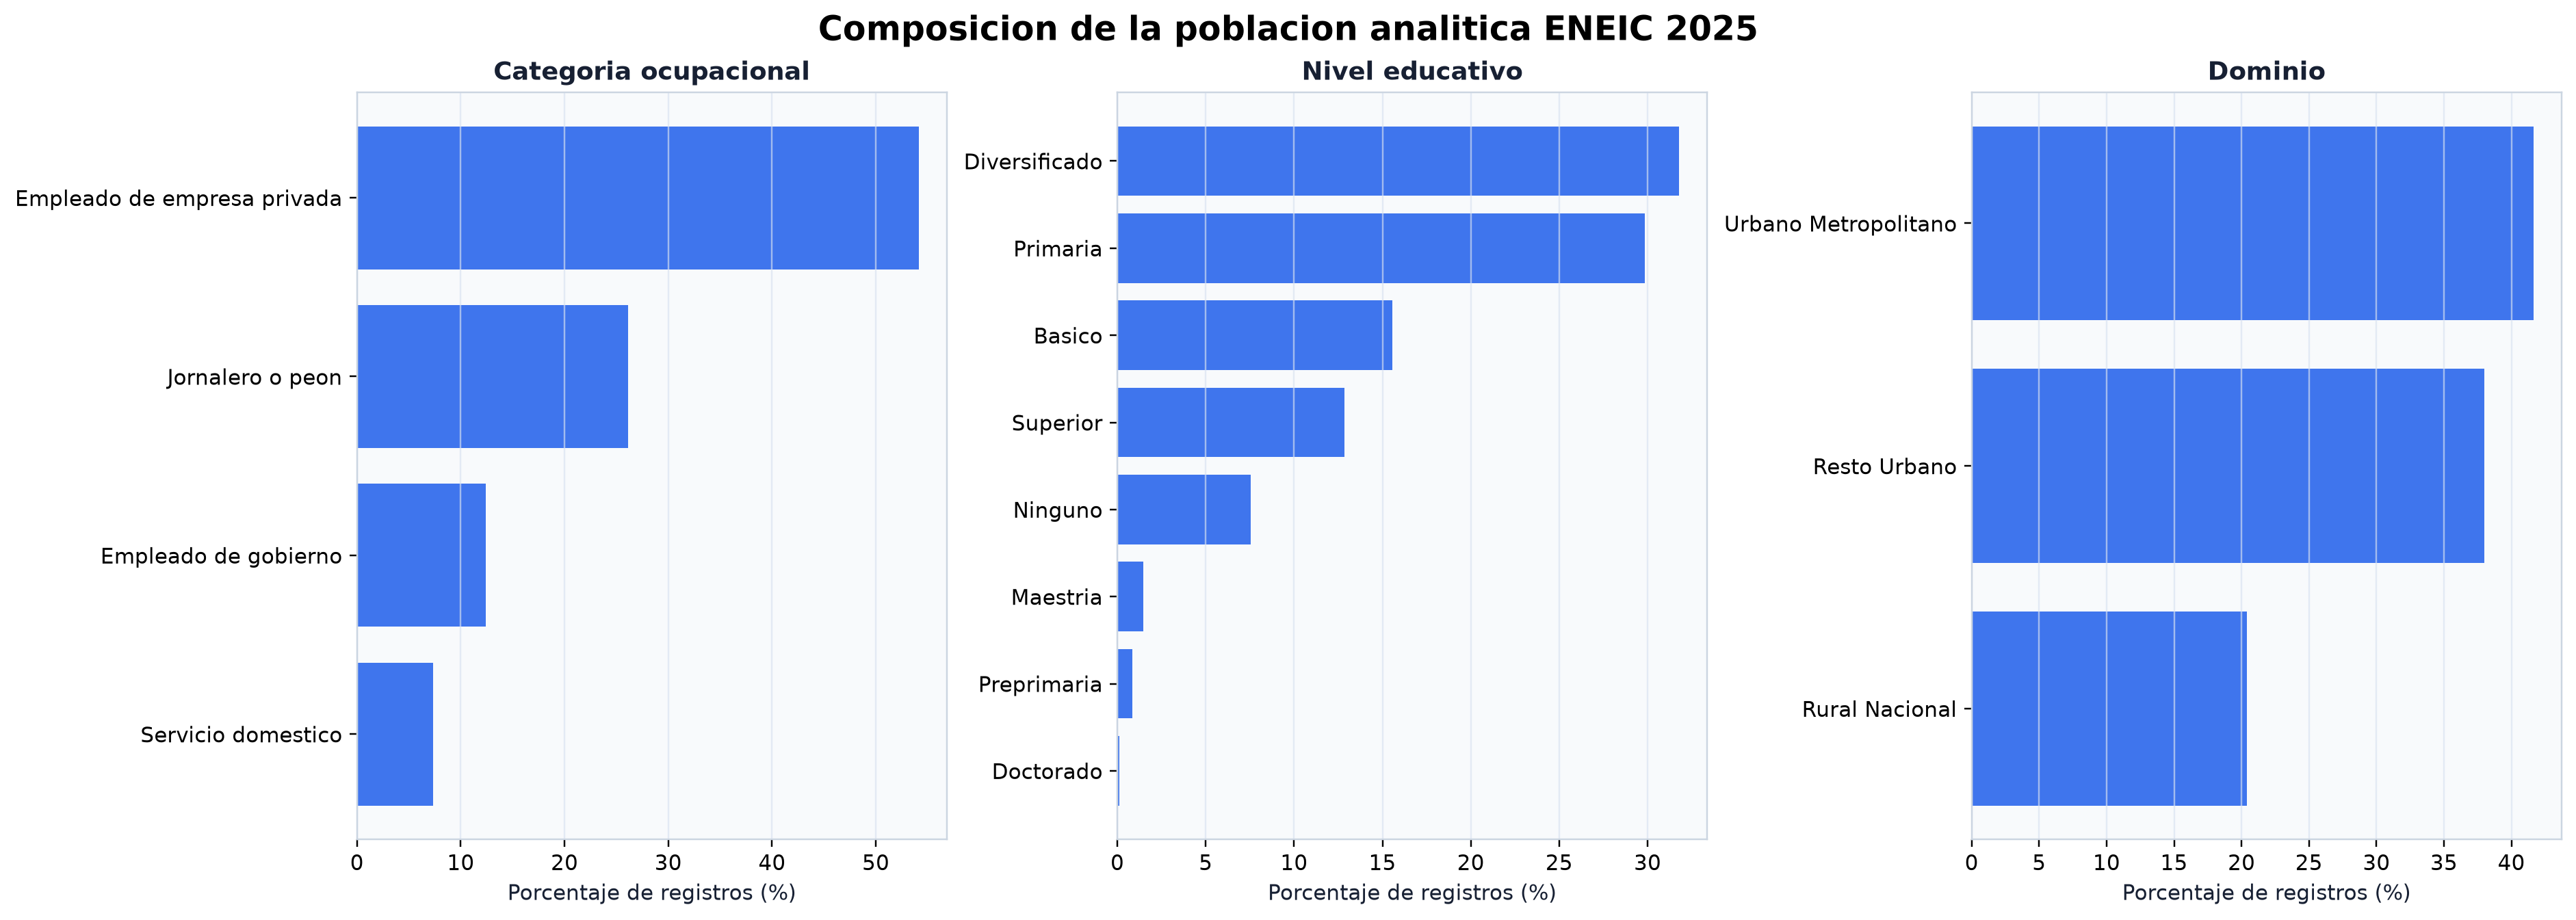
\includegraphics[width=0.96\textwidth]{distribuciones_categoricas.png}
\caption{Composición de los registros elegibles de 2025.}
\end{figure}

\begin{figure}[htbp]
\centering
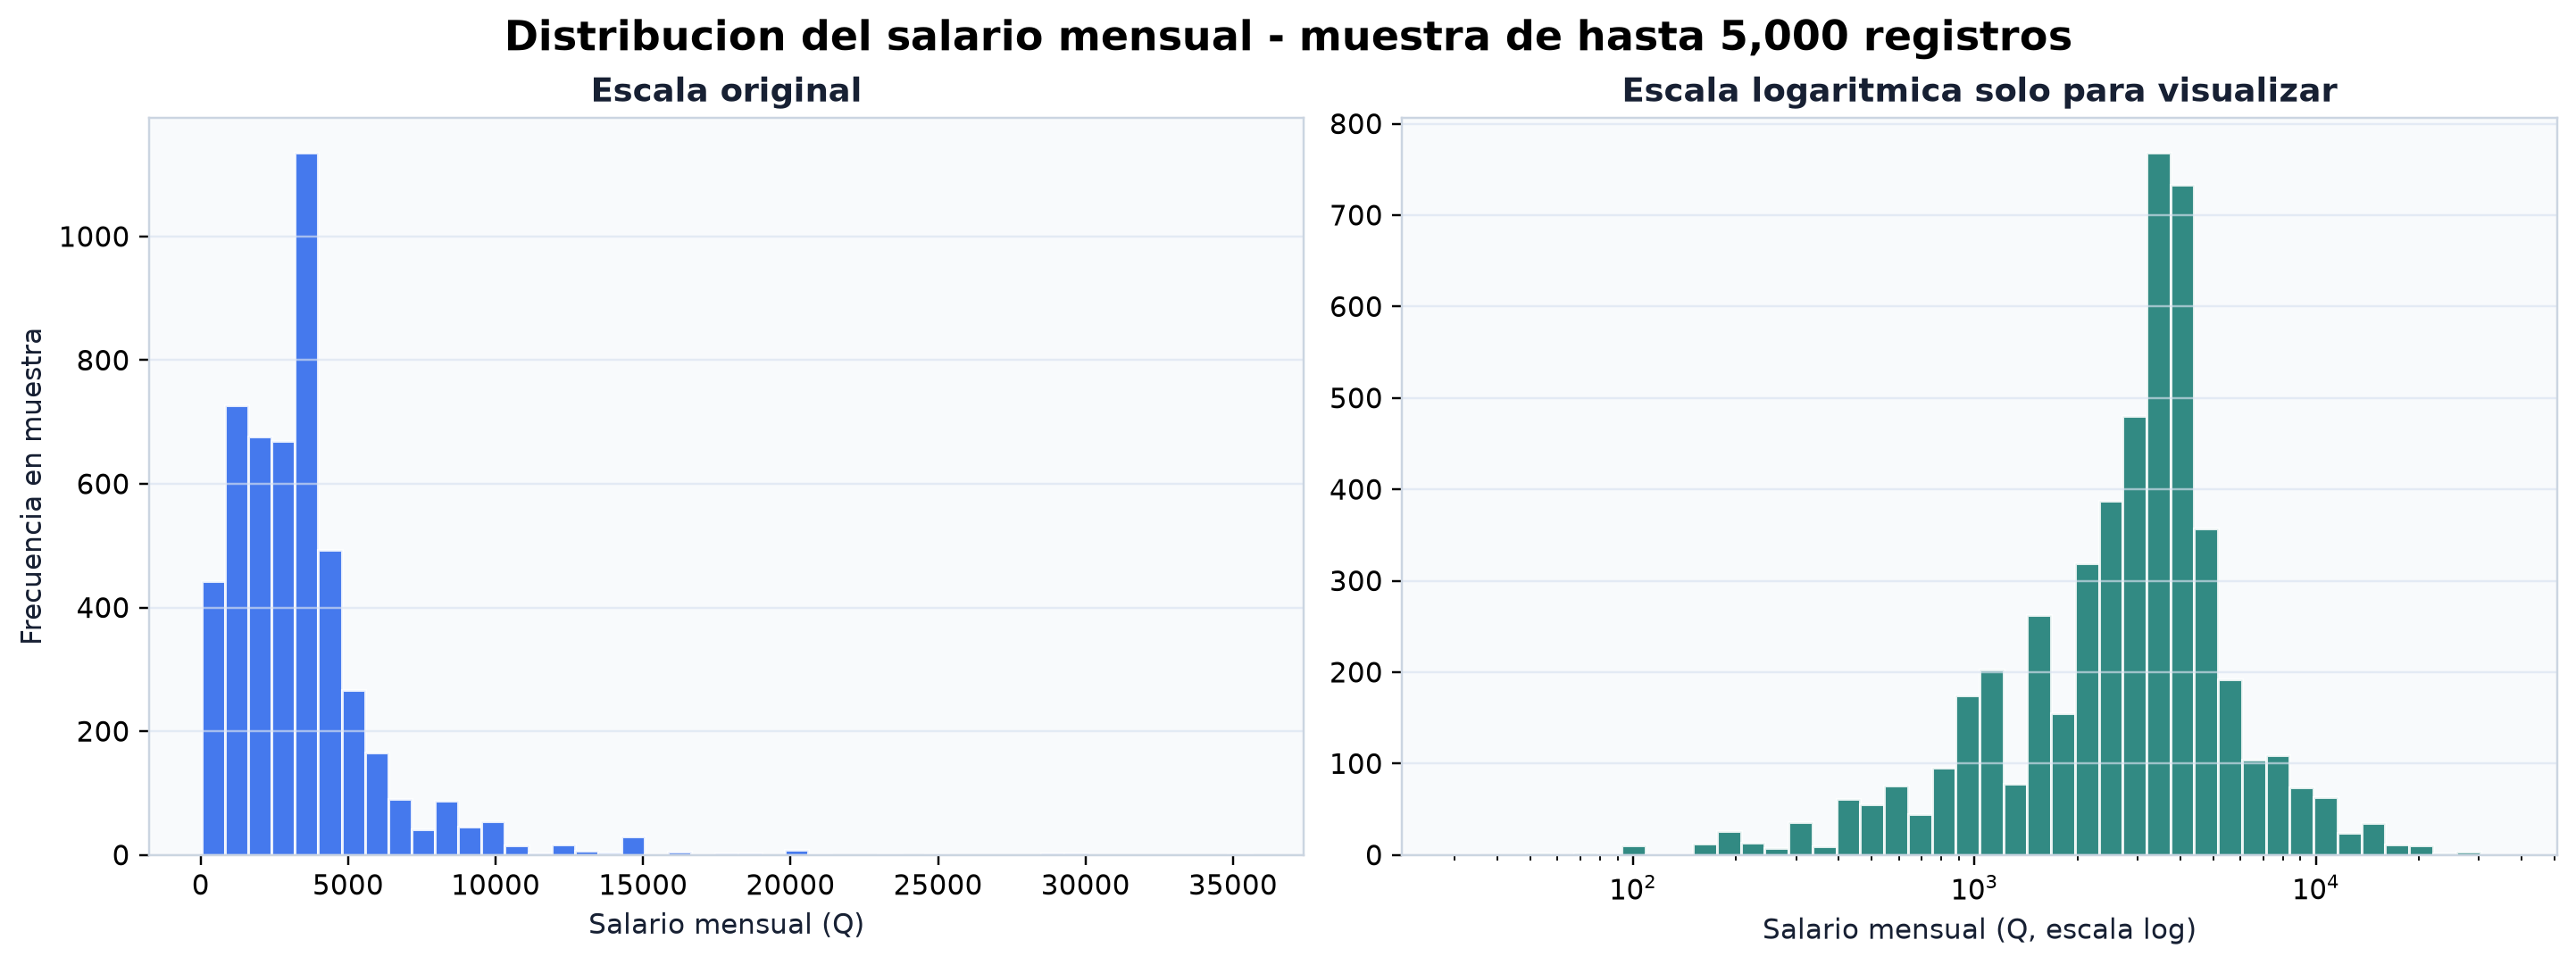
\includegraphics[width=0.96\textwidth]{distribucion_salario.png}
\caption{Distribución salarial; la escala logarítmica se usa únicamente para visualizar.}
\end{figure}

\begin{figure}[htbp]
\centering
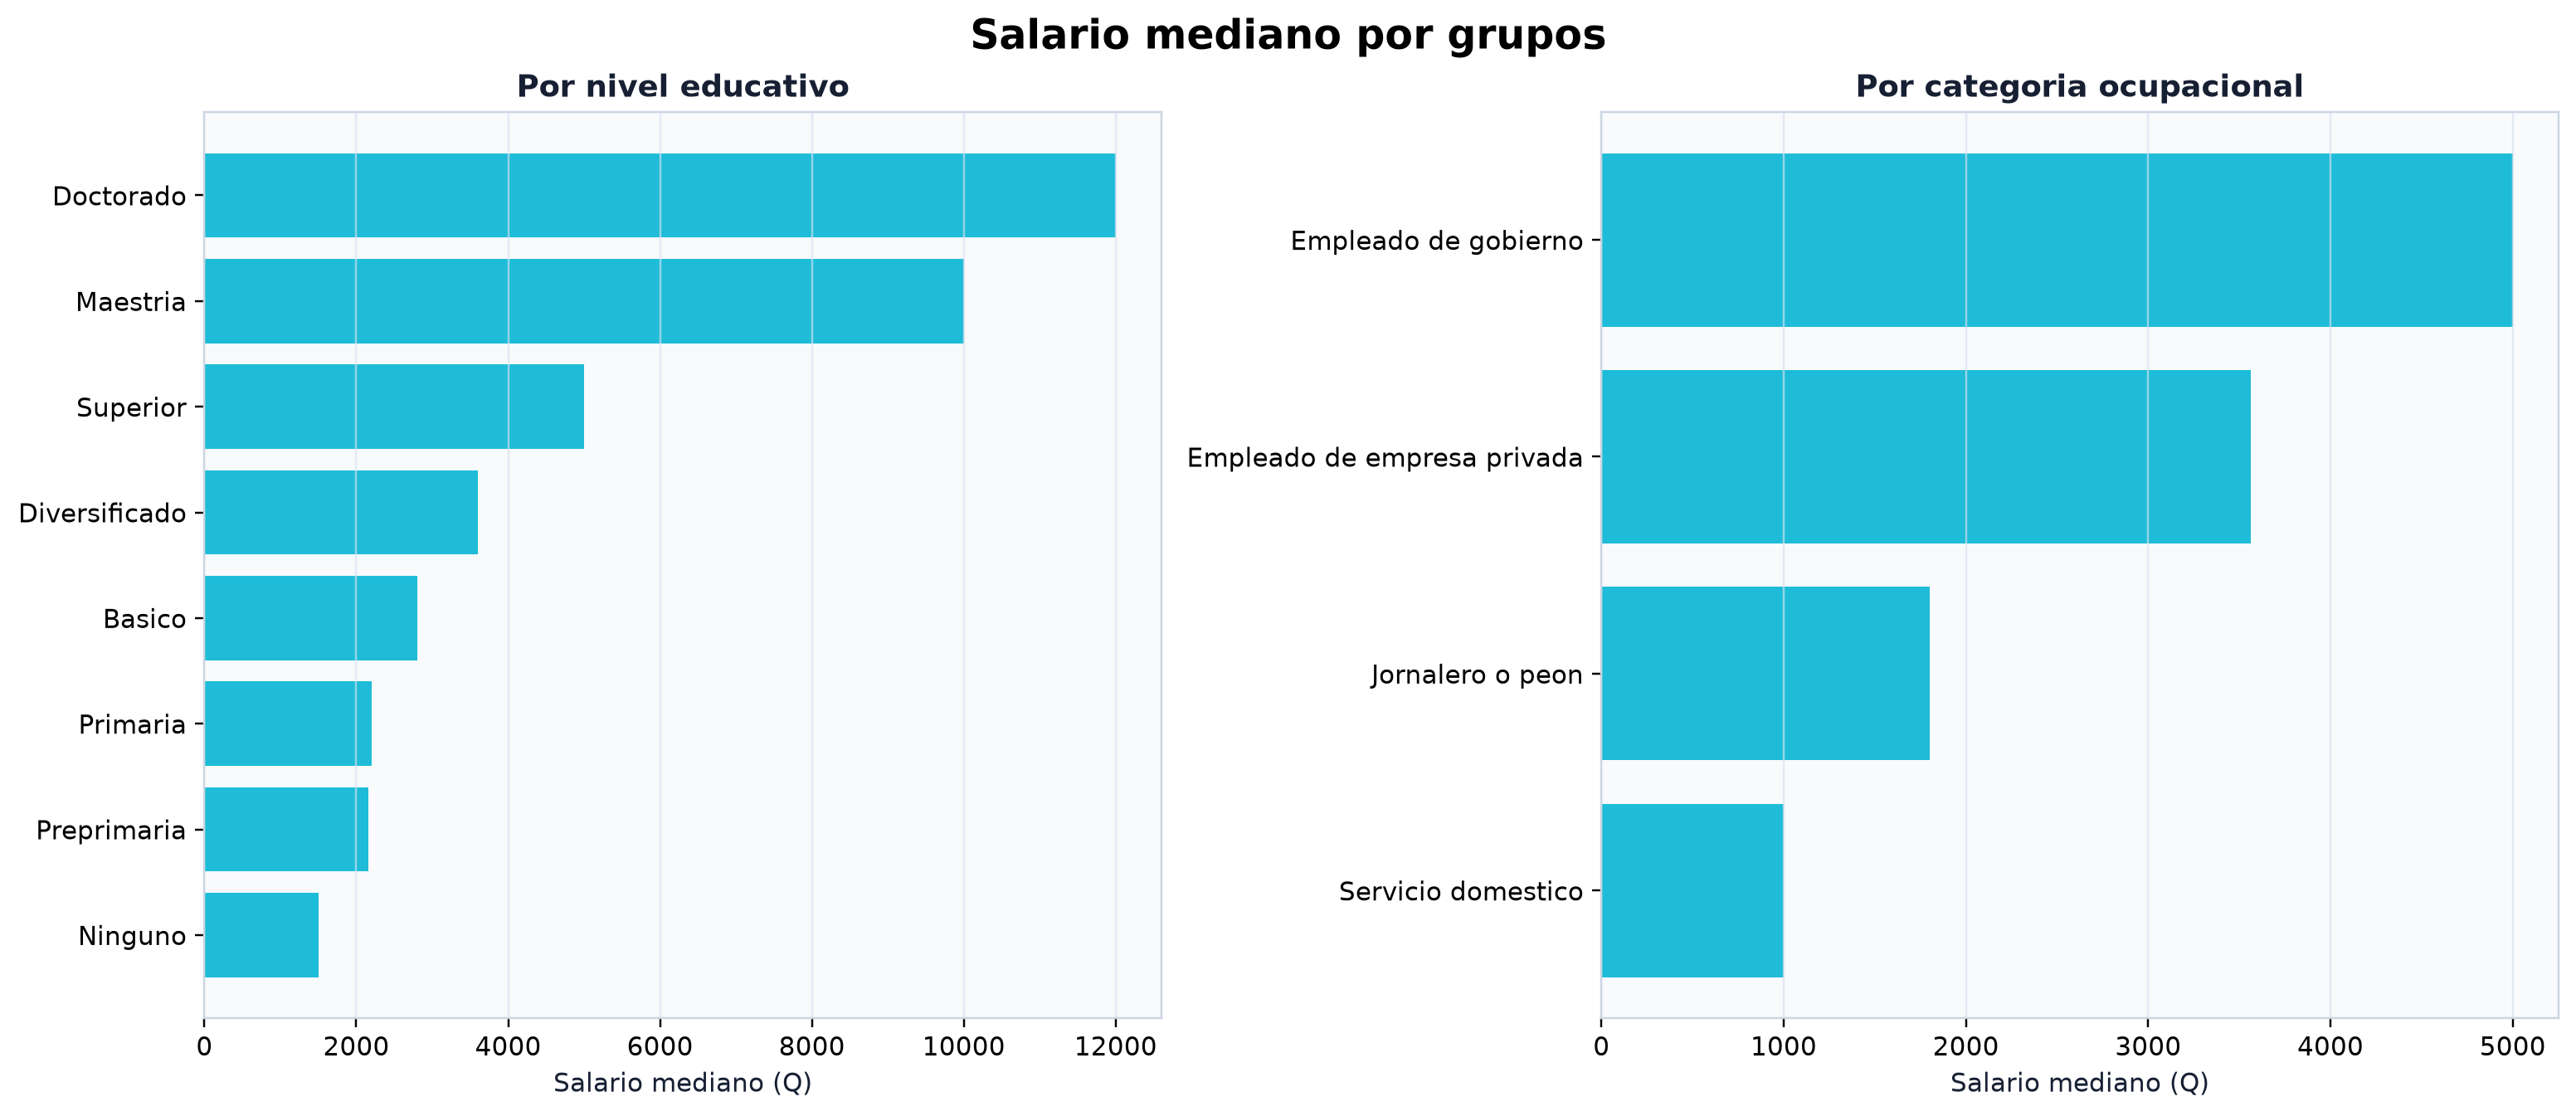
\includegraphics[width=0.90\textwidth]{salario_mediano_grupos.png}
\caption{Salario mediano por educación y categoría ocupacional.}
\end{figure}

\begin{figure}[htbp]
\centering
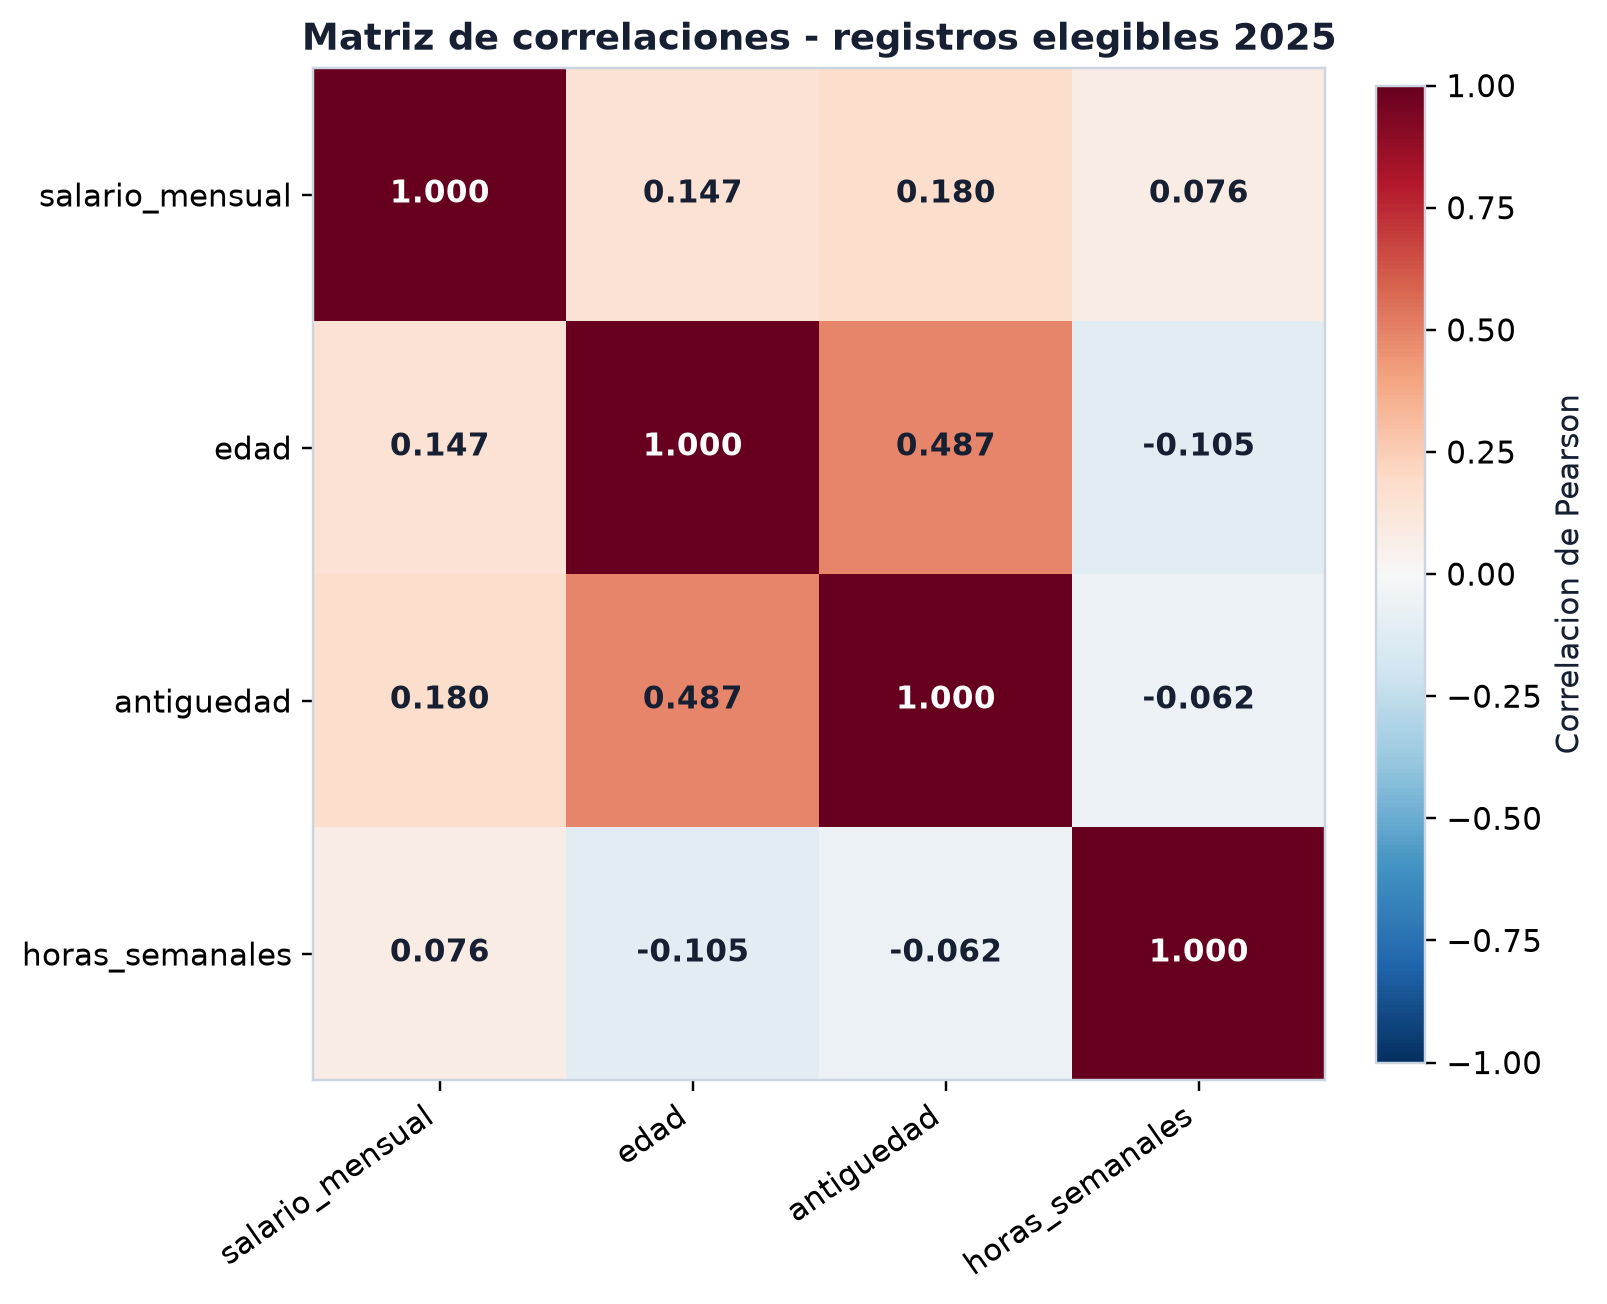
\includegraphics[width=0.78\textwidth]{correlaciones_pearson.png}
\caption{Correlaciones de Pearson calculadas sobre todos los registros elegibles de 2025.}
\end{figure}

\section{Segmentación y validación de modelos}

KMeans comparó $K=2,3,4,5$ con variables estandarizadas, tanto con un perfil
laboral sin salario como con un perfil económico que sí lo incorpora. Para el
modelado supervisado se utilizaron exactamente edad, antigüedad, horas
semanales, educación, categoría ocupacional y dominio.

\begin{figure}[htbp]
\centering
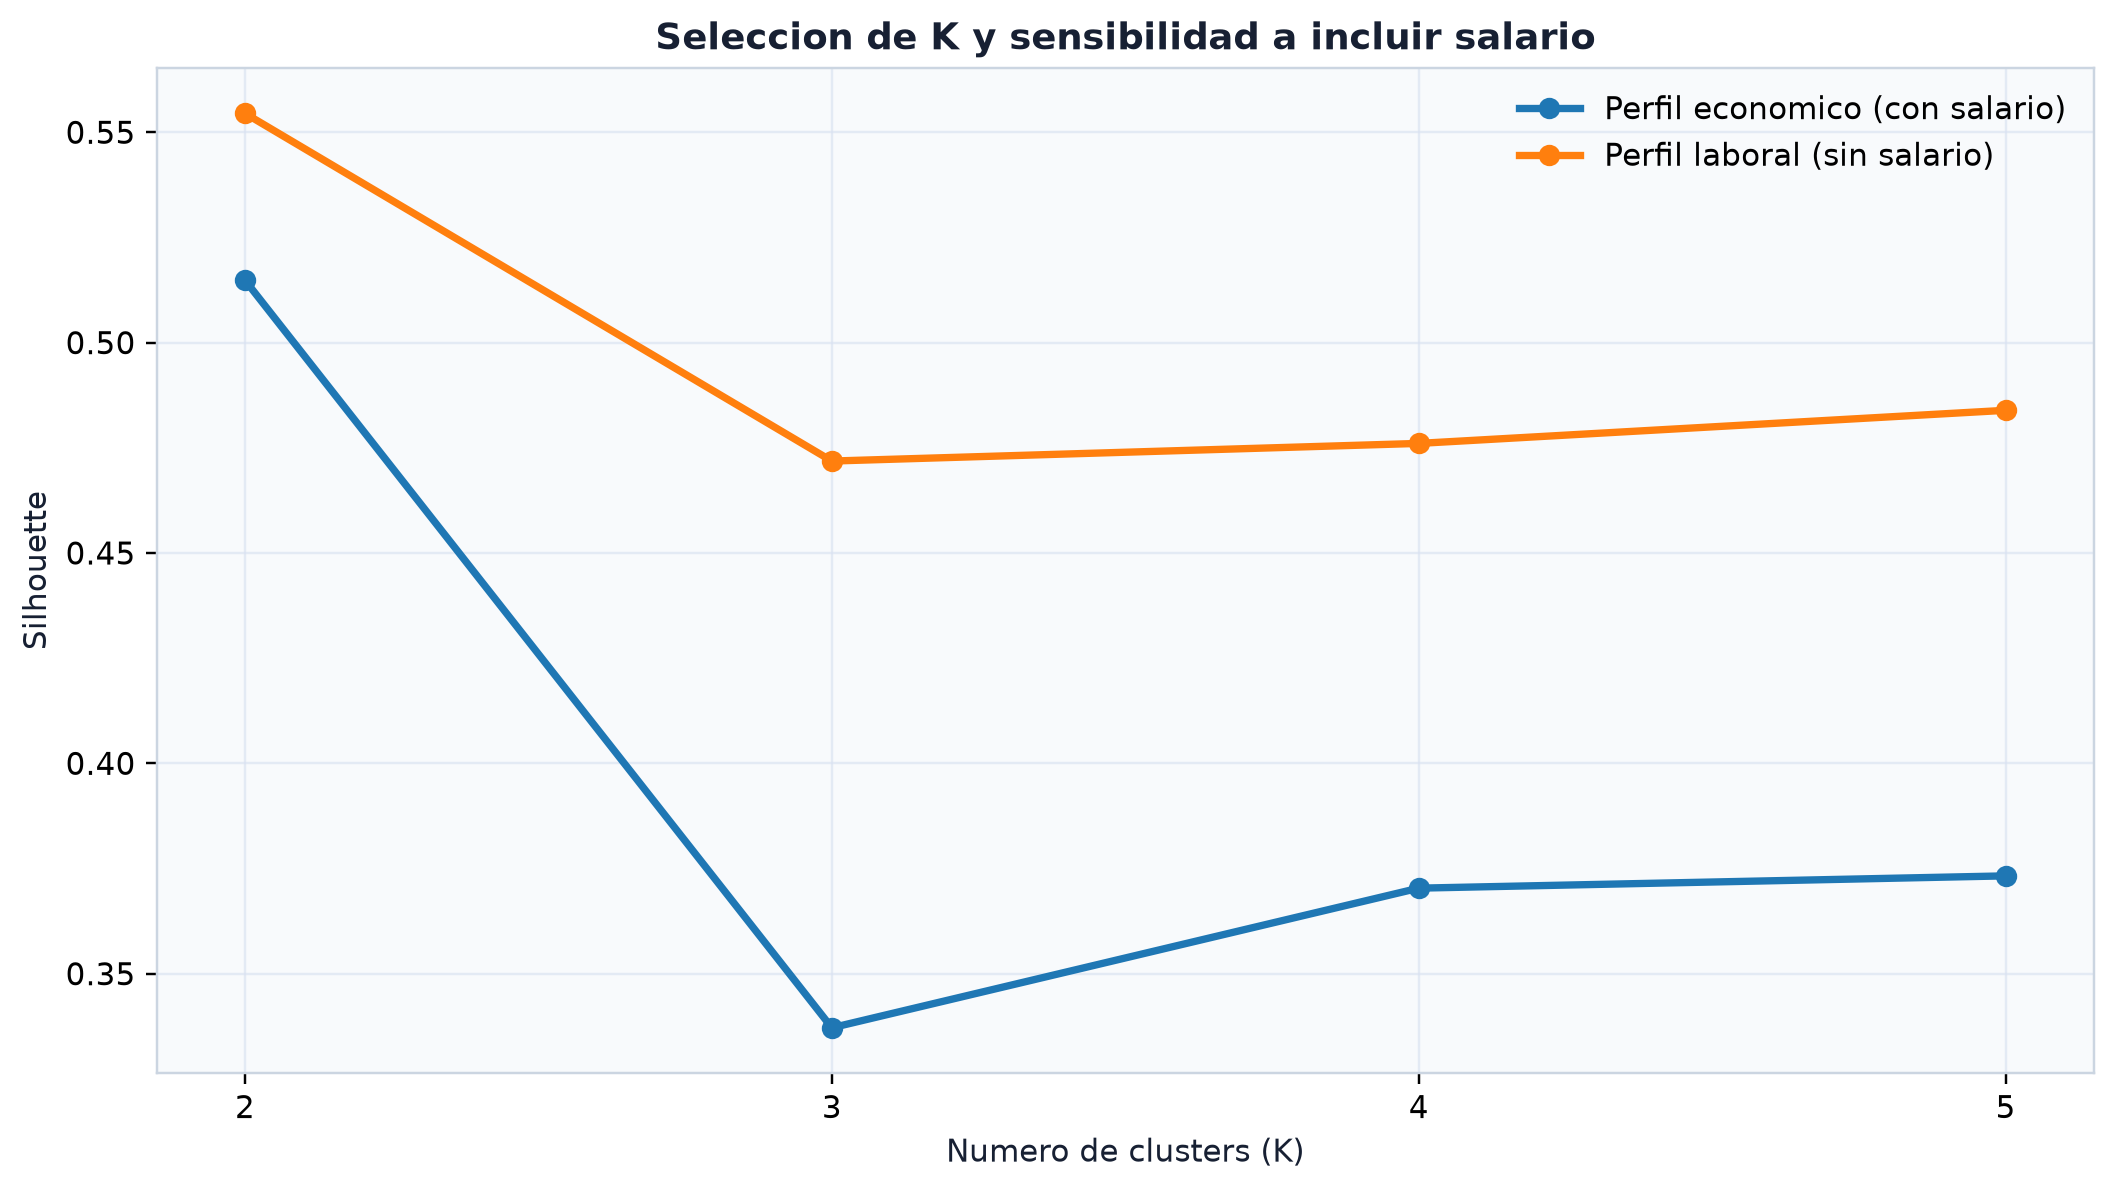
\includegraphics[width=0.82\textwidth]{seleccion_kmeans.png}
\caption{Selección de K y sensibilidad a incluir el salario.}
\end{figure}

\begin{figure}[htbp]
\centering
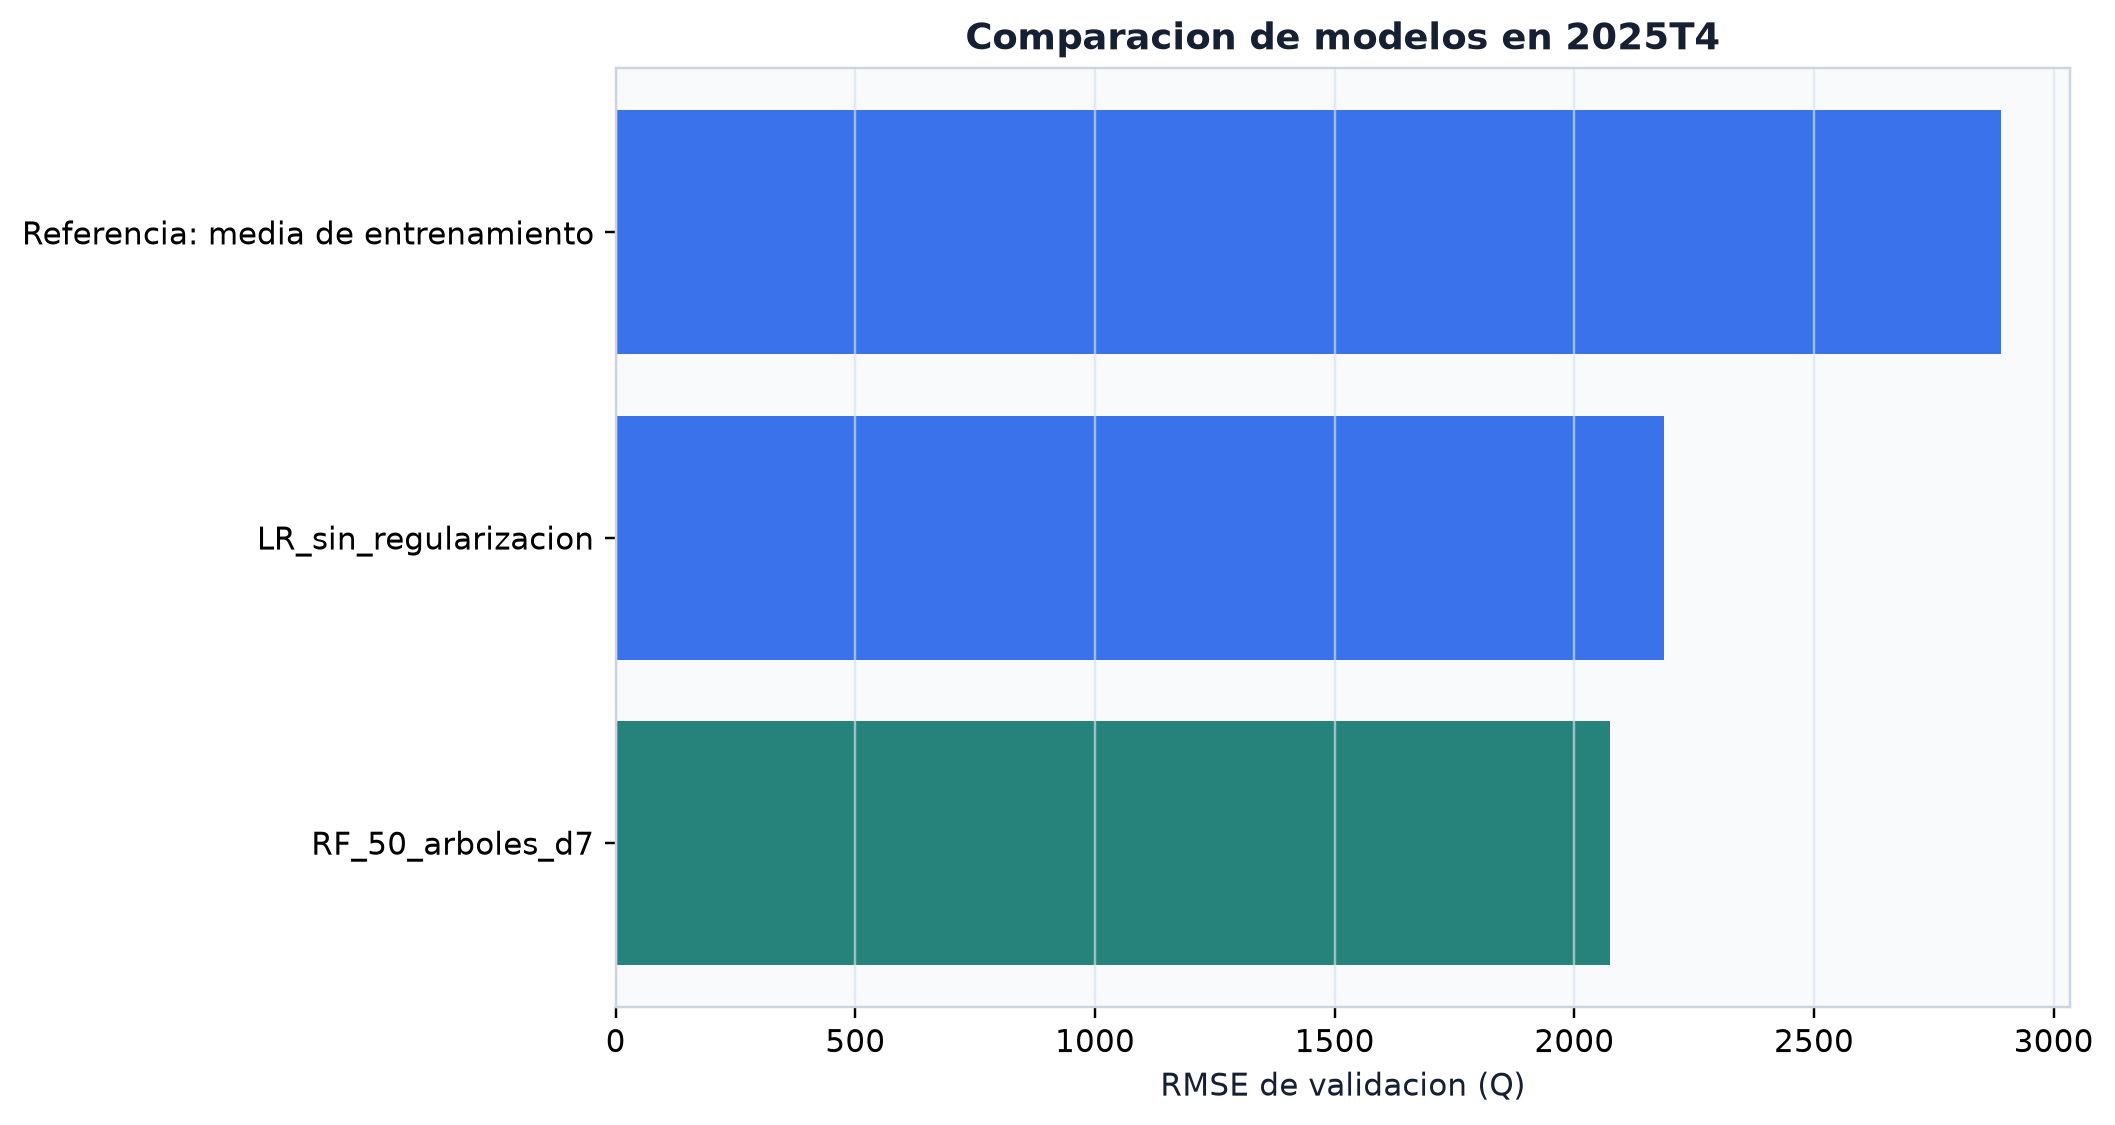
\includegraphics[width=0.86\textwidth]{comparacion_modelos_validacion.png}
\caption{Comparación de RMSE en validación temporal 2025T4.}
\end{figure}

\section{Evaluación final en 2026T1}

Los pipelines completos se reajustaron con 2025T1--T4. Ambos modelos se
evaluaron sobre las mismas claves elegibles de 2026T1, sin seleccionar de
nuevo hiperparámetros.

\begin{table}[htbp]\centering\footnotesize
\begin{tabular}{llrrrr}\toprule
Modelo & Configuración & Registros & MAE (Q) & RMSE (Q) & $R^2$ \\ \midrule
RF\_50\_arboles\_d7 & numTrees=50, maxDepth=7 & 13,258 & 1,141.51 & 2,050.55 & 0.4887 \\
LR\_sin\_regularizacion & regParam=0.0, elasticNetParam=0.0 & 13,258 & 1,240.71 & 2,163.75 & 0.4307 \\
Referencia: media 2025 & media salarial 2025 completo & 13,258 & 1,718.09 & 2,871.42 & -0.0025 \\
\bottomrule\end{tabular}
\caption{Métricas en 2026T1, no ponderadas y calculadas sobre todo el conjunto de prueba.}
\end{table}
\begin{table}[htbp]\centering\small
\begin{tabular}{lr}\toprule
Conjunto & Registros \\ \midrule
Test elegible 2026T1 & 13,258 \\
Predicciones LR\_sin\_regularizacion & 13,258 \\
Predicciones RF\_50\_arboles\_d7 & 13,258 \\
Registros compartidos (join por clave) & 13,258 \\
Claves distintas compartidas & 13,258 \\
\bottomrule\end{tabular}
\caption{Ambos modelos se evalúan sobre exactamente los mismos registros (misma clave y mismo conteo).}
\end{table}
\begin{table}[htbp]\centering\footnotesize
\begin{tabular}{lrrrr}\toprule
Modelo & RMSE 2025T4 & RMSE 2026T1 & Cambio & Mejora vs. referencia \\ \midrule
RF\_50\_arboles\_d7 & 2,074.15 & 2,050.55 & -23.60 & 28.59\% \\
LR\_sin\_regularizacion & 2,186.42 & 2,163.75 & -22.67 & 24.65\% \\
Referencia: media 2025 & 2,889.57 & 2,871.42 & -18.15 & 0.00\% \\
\bottomrule\end{tabular}
\caption{Estabilidad temporal del RMSE y mejora frente a la referencia de la media de 2025.}
\end{table}

En 2026T1, \textbf{RF\_50\_arboles\_d7} obtuvo el menor error (MAE Q1,141.51, RMSE Q2,050.55, $R^2$ 0.4887); el otro algoritmo, \textbf{LR\_sin\_regularizacion}, obtuvo MAE Q1,240.71, RMSE Q2,163.75 y $R^2$ 0.4307. La referencia (media de 2025) tiene RMSE Q2,871.42 y $R^2$ -0.0025, y el ganador reduce ese RMSE en 28.59\%. El ganador de validación coincide con el de prueba.


\section{Visualización y análisis de errores}

Se definió el residuo como salario real menos salario predicho: un valor
positivo indica subestimación y uno negativo, sobreestimación. Los diagramas
usan la misma muestra reproducible de 5,000 registros; las métricas por grupo
se calcularon con el test completo.

\textbf{Resultados globales (todo el test).}

\begin{itemize}\setlength{\itemsep}{2pt}
\item \textbf{Random Forest:} error medio global +107.45 Q (subestima en promedio); subestima al 47.0\% de los registros.
\item \textbf{Regresión lineal:} error medio global +120.55 Q (subestima en promedio); subestima al 48.9\% de los registros.
\end{itemize}

\textbf{Lo que muestran las gráficas (muestra común de 5,000 registros).}

\begin{itemize}\setlength{\itemsep}{2pt}
\item \textbf{Regresion lineal:} en la muestra, el residuo medio es Q105.62; para salarios reales desde el percentil 90 es Q3,282.91. La dispersion crece con el nivel salarial, por lo que los errores no tienen varianza constante.
\item \textbf{Random Forest:} en la muestra, el residuo medio es Q95.47; para salarios reales desde el percentil 90 es Q3,202.76. La dispersion crece con el nivel salarial, por lo que los errores no tienen varianza constante.
\end{itemize}


\begin{figure}[htbp]
\centering
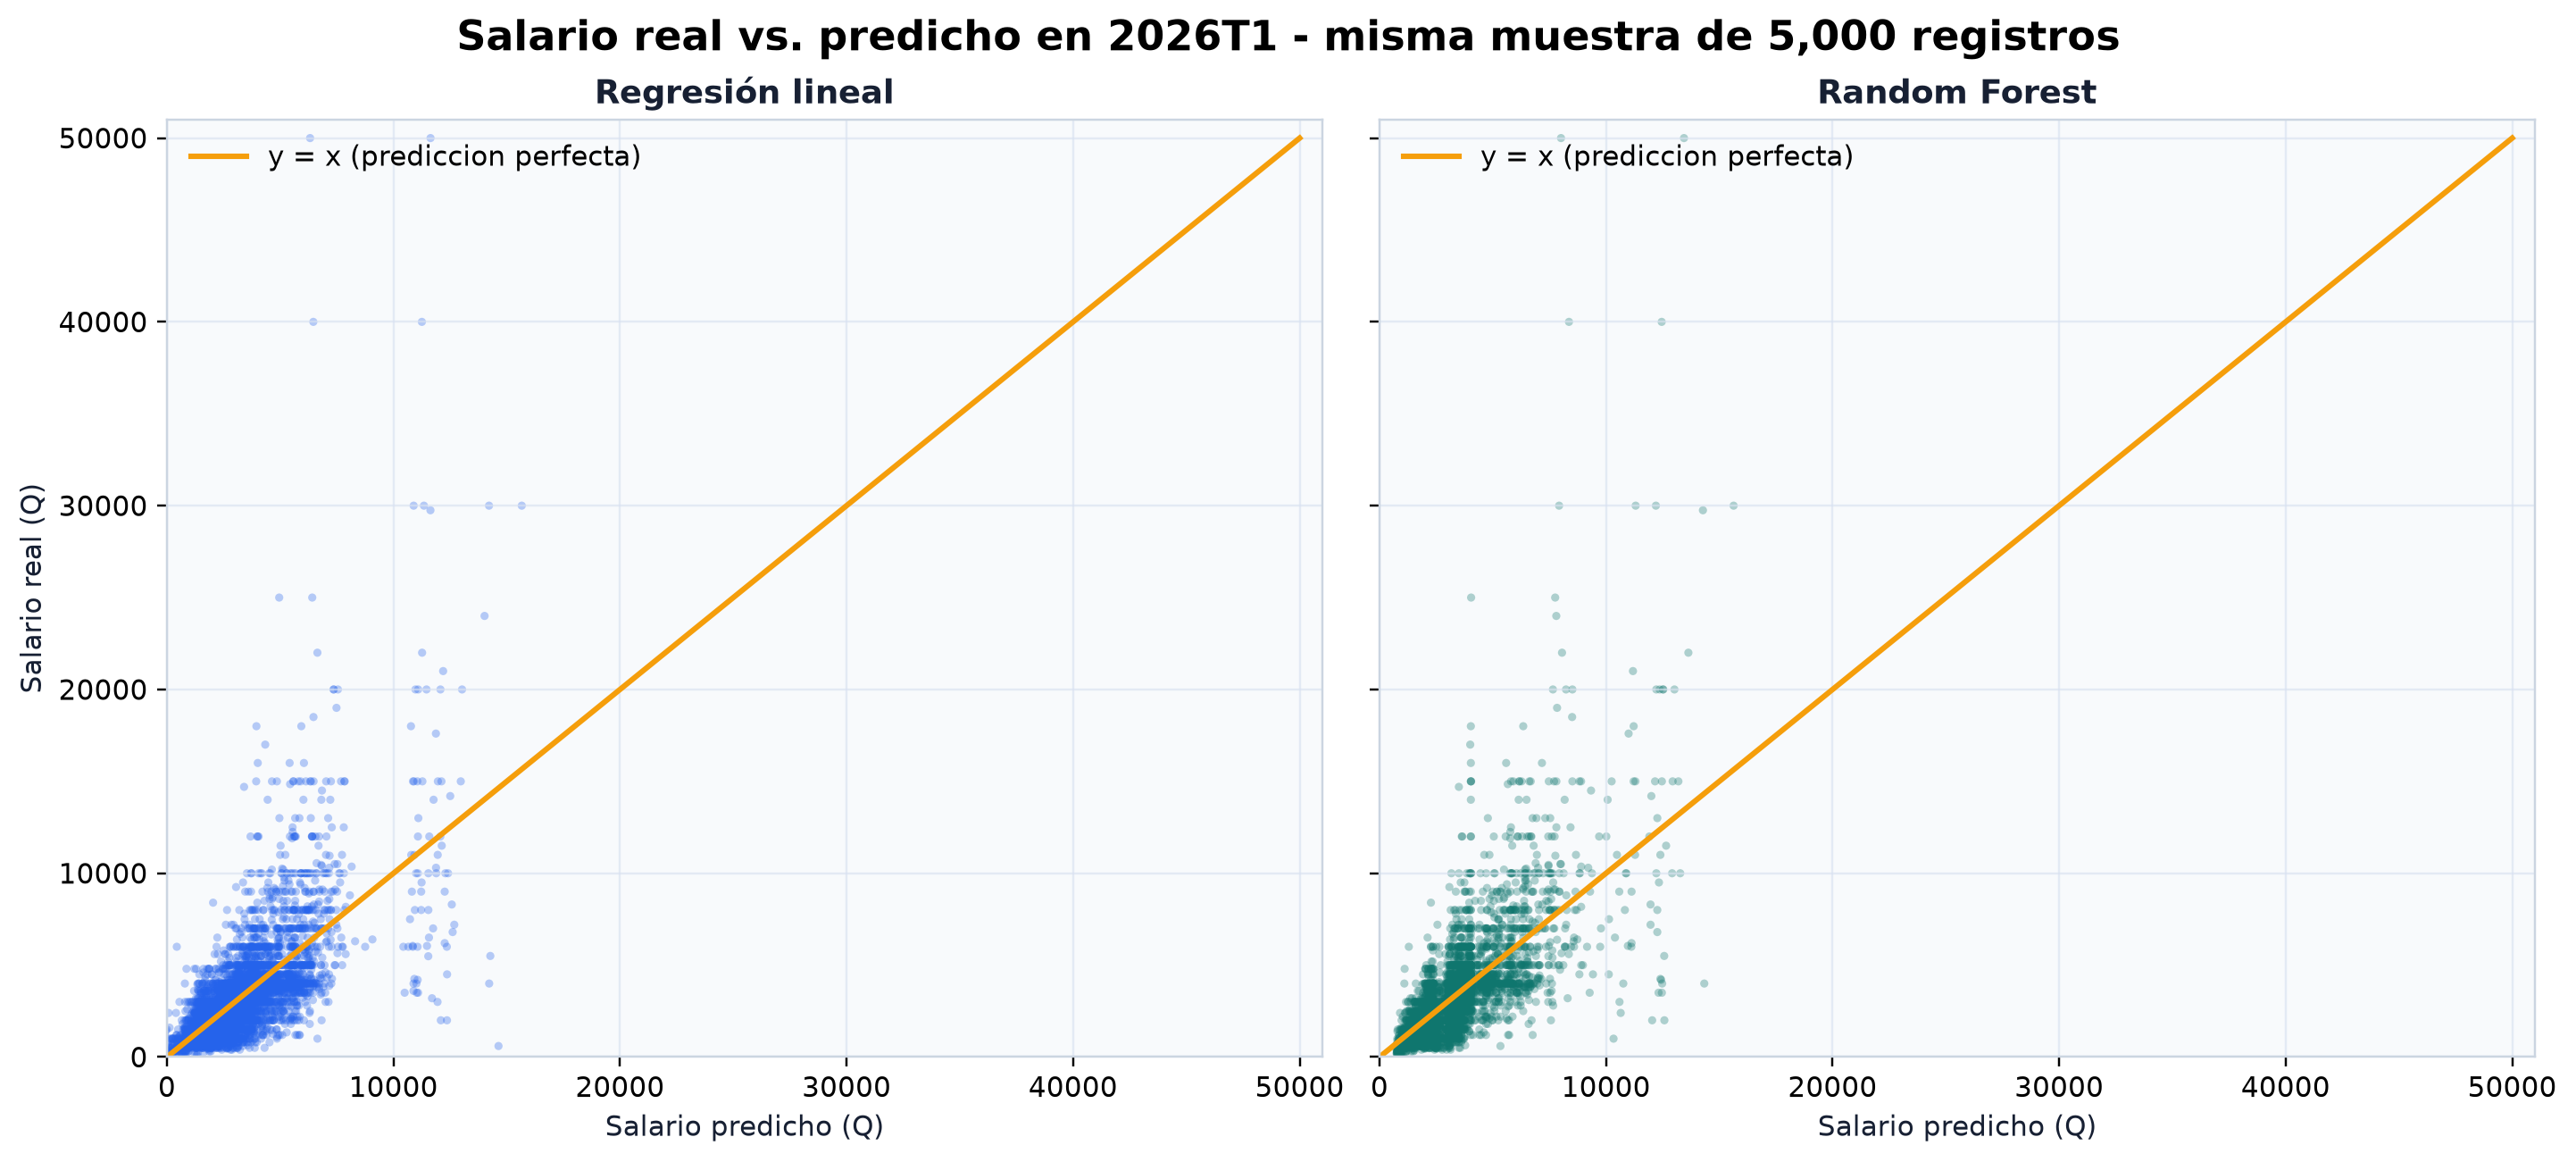
\includegraphics[width=\textwidth]{real_vs_predicho_2026.png}
\caption{Salario real frente a predicho con referencia $y=x$.}
\end{figure}

\begin{figure}[htbp]
\centering
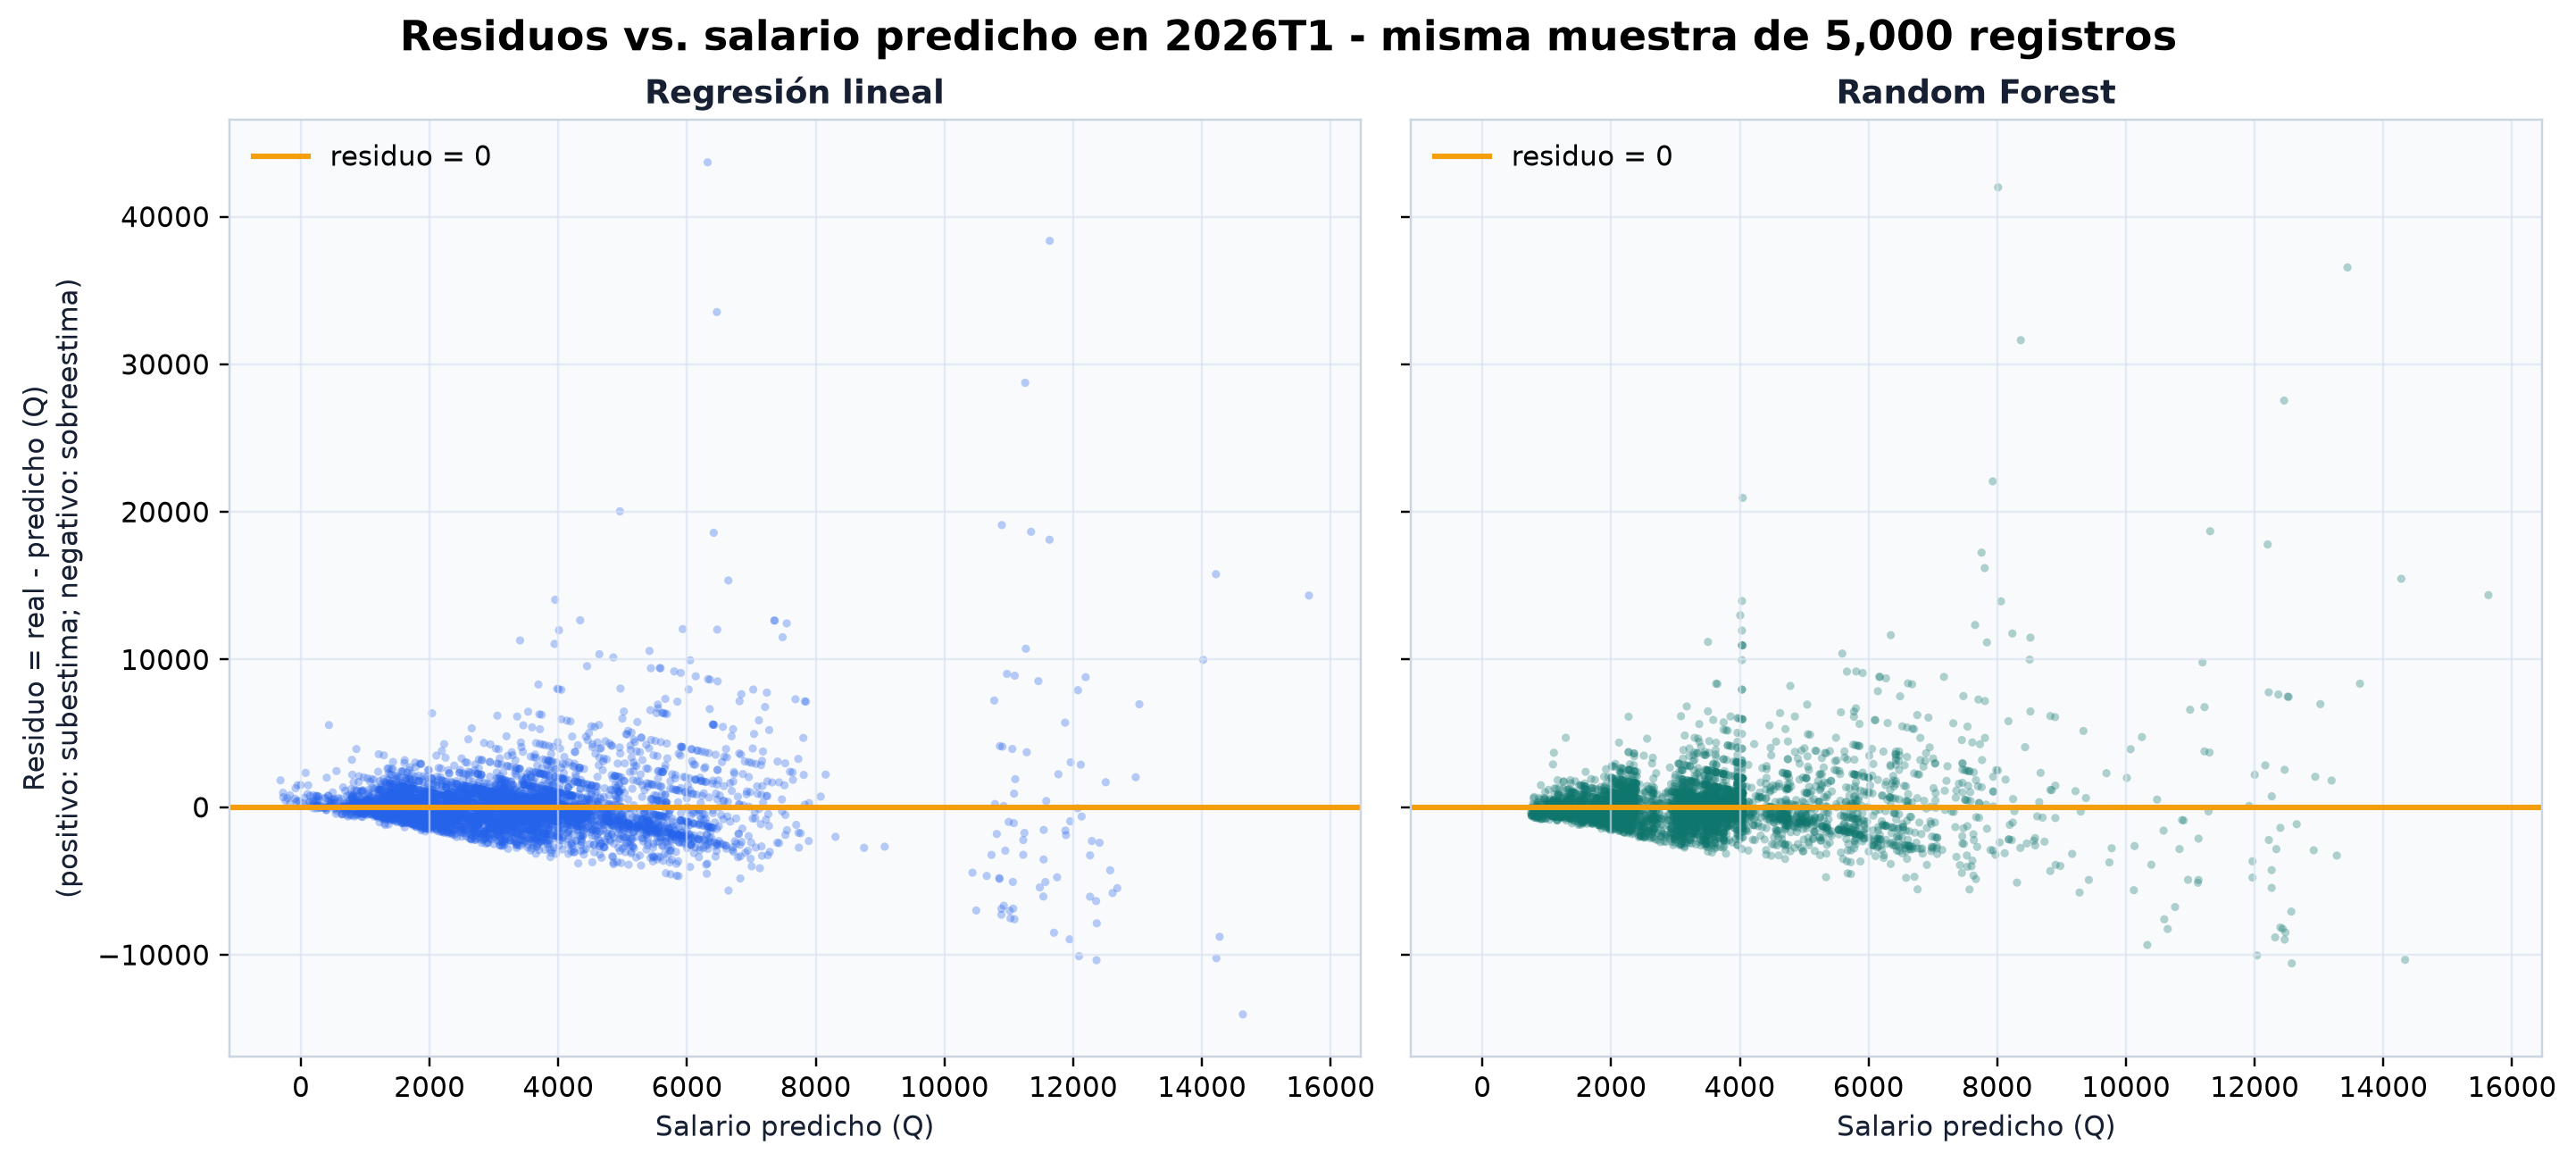
\includegraphics[width=\textwidth]{residuos_vs_predicho_2026.png}
\caption{Residuos frente a predicción con referencia horizontal en cero.}
\end{figure}

\subsection{Errores por nivel educativo}
\begin{table}[htbp]\centering\footnotesize
\begin{tabular}{lrrrrr}\toprule
Nivel educativo & n & MAE RL & Err. medio RL & MAE RF & Err. medio RF \\ \midrule
Ninguno & 1,016 & 823.51 & +109.34 & 708.92 & -197.02 \\
Preprimaria & 80 & 735.21 & +88.76 & 661.81 & -192.45 \\
Primaria & 3,957 & 870.04 & +54.56 & 777.34 & -6.77 \\
Basico & 2,164 & 894.45 & +127.77 & 850.43 & +54.88 \\
Diversificado & 4,117 & 1,109.31 & +103.98 & 1,045.38 & +200.09 \\
Superior & 1,729 & 2,566.37 & +295.51 & 2,358.83 & +342.58 \\
Maestria & 183 & 5,552.88 & -131.50 & 4,882.13 & +39.54 \\
Doctorado & 12 & 12,919.31 & +6,062.70 & 14,088.18 & +10,397.51 \\
\bottomrule\end{tabular}
\caption{MAE y error medio (real $-$ predicho) por nivel educativo; RL = regresión lineal, RF = Random Forest.}
\end{table}
\begin{itemize}\setlength{\itemsep}{2pt}
\item \textbf{Random Forest:} el mayor MAE por nivel educativo aparece en \textbf{Doctorado} (Q14,088.18, n=12). La mayor subestimación media ocurre en \textbf{Doctorado} (Q10,397.51) y la mayor sobreestimación ocurre en \textbf{Ninguno} (Q-197.02).
\item \textbf{Regresión lineal:} el mayor MAE por nivel educativo aparece en \textbf{Doctorado} (Q12,919.31, n=12). La mayor subestimación media ocurre en \textbf{Doctorado} (Q6,062.70) y la mayor sobreestimación ocurre en \textbf{Maestria} (Q-131.50).
\end{itemize}

El grupo de nivel educativo con mayor salario promedio es \textbf{Doctorado} (Q20,291.67) y tambien concentra el mayor MAE absoluto; esto obliga a interpretar el MAE junto con la escala salarial y el numero de observaciones.

\subsection{Errores por dominio}
\begin{table}[htbp]\centering\footnotesize
\begin{tabular}{lrrrrr}\toprule
Dominio & n & MAE RL & Err. medio RL & MAE RF & Err. medio RF \\ \midrule
Resto Urbano & 4,846 & 1,189.65 & +134.28 & 1,085.55 & +66.32 \\
Rural Nacional & 2,780 & 913.64 & +65.24 & 813.65 & -62.41 \\
Urbano Metropolitano & 5,632 & 1,446.09 & +136.04 & 1,351.50 & +226.68 \\
\bottomrule\end{tabular}
\caption{MAE y error medio (real $-$ predicho) por dominio; RL = regresión lineal, RF = Random Forest.}
\end{table}
\begin{itemize}\setlength{\itemsep}{2pt}
\item \textbf{Random Forest:} el mayor MAE por dominio aparece en \textbf{Urbano Metropolitano} (Q1,351.50, n=5,632). La mayor subestimación media ocurre en \textbf{Urbano Metropolitano} (Q226.68) y la mayor sobreestimación ocurre en \textbf{Rural Nacional} (Q-62.41).
\item \textbf{Regresión lineal:} el mayor MAE por dominio aparece en \textbf{Urbano Metropolitano} (Q1,446.09, n=5,632). La mayor subestimación media ocurre en \textbf{Urbano Metropolitano} (Q136.04) y todos los grupos presentan subestimación media; la menor aparece en \textbf{Rural Nacional} (Q65.24).
\end{itemize}

El grupo de dominio con mayor salario promedio es \textbf{Urbano Metropolitano} (Q4,352.31) y tambien concentra el mayor MAE absoluto; esto obliga a interpretar el MAE junto con la escala salarial y el numero de observaciones.

\subsection{Errores según el percentil del salario real}
\begin{table}[htbp]\centering\footnotesize
\begin{tabular}{lrrrrrrr}\toprule
Banda & n & Salario prom. & MAE RL & Err. RL & MAE RF & Err. RF & RF subestima \\ \midrule
P00-P25 & 4,032 & 1,298 & 998 & -829 & 928 & -868 & 10.9\% \\
P25-P50 & 2,715 & 2,738 & 852 & -161 & 701 & -209 & 42.5\% \\
P50-P75 & 3,188 & 3,769 & 831 & -80 & 691 & -26 & 60.5\% \\
P75-P90 & 2,072 & 4,889 & 1,178 & +486 & 1,200 & +551 & 75.3\% \\
P90-P95 & 608 & 7,225 & 2,076 & +1,634 & 2,048 & +1,644 & 88.3\% \\
P95-P100 & 643 & 12,553 & 5,848 & +5,645 & 5,524 & +5,341 & 94.4\% \\
\bottomrule\end{tabular}
\caption{Error por banda del salario real de 2026T1 (todos los registros de prueba); error = real $-$ predicho.}
\end{table}
\begin{itemize}\setlength{\itemsep}{2pt}
\item \textbf{Random Forest:} en P00-P25 el error medio es Q-868.49; en P95-P100 asciende a Q5,341.04, con MAE Q5,524.16 y 94.4\% de registros subestimados.
\item \textbf{Regresión lineal:} en P00-P25 el error medio es Q-828.73; en P95-P100 asciende a Q5,645.34, con MAE Q5,848.39 y 94.4\% de registros subestimados.
\end{itemize}

\textbf{Salarios bajos, medios y altos.} \textbf{RF\_50\_arboles\_d7} es el mejor modelo global por RMSE. Sin embargo, en P95-P100 todavia presenta un error medio de Q5,341.04 y un MAE de Q5,524.16; por tanto, una mejora promedio no elimina la dificultad de representar la cola salarial.

\subsection{Respuestas a las preguntas de la actividad}
\begin{itemize}\setlength{\itemsep}{2pt}
\item \textbf{Algoritmo con mejor generalizacion:} RF\_50\_arboles\_d7, con RMSE Q2,050.55 y $R^2$=0.4887, frente a RMSE Q2,163.75 del otro algoritmo.
\item \textbf{Nivel educativo con mayor error observado:} Doctorado para Random Forest (MAE Q14,088.18, n=12).
\item \textbf{Dominio con mayor error observado:} Urbano Metropolitano para Regresión lineal (MAE Q1,446.09, n=5,632).
\item \textbf{Banda mas dificil:} P95-P100 para Regresión lineal (MAE Q5,848.39). Los errores medios positivos en la cola alta indican subestimacion sistematica de salarios altos.
\item \textbf{Lectura correcta:} las diferencias son predictivas y descriptivas; no prueban causalidad ni determinan cuanto deberia ganar una persona.
\end{itemize}


\begin{figure}[htbp]
\centering
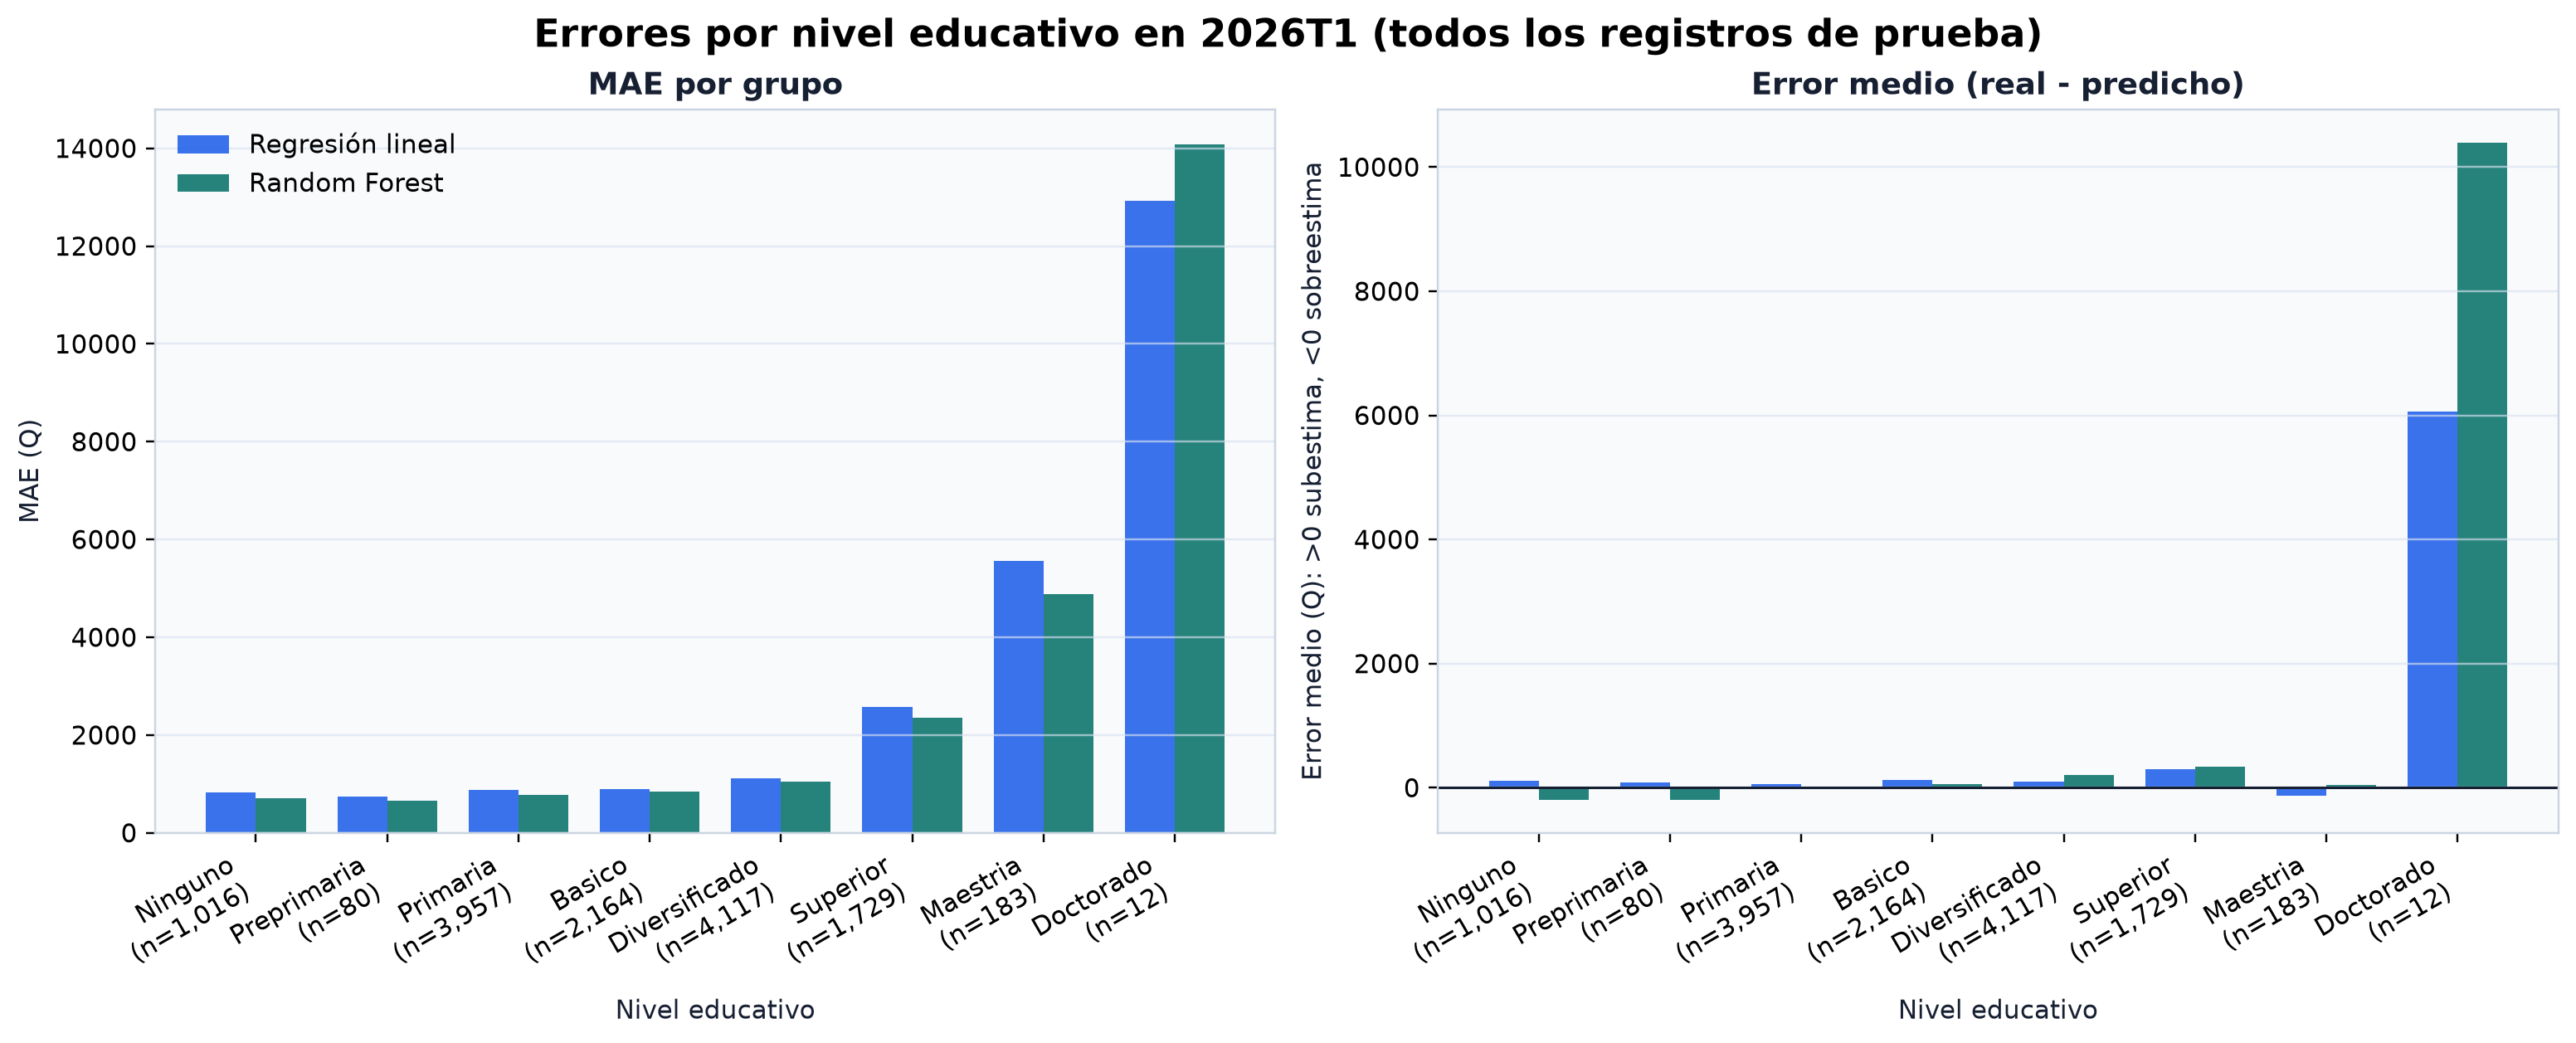
\includegraphics[width=\textwidth]{errores_por_educacion_2026.png}
\caption{MAE y error medio por nivel educativo sobre todo el test.}
\end{figure}

\begin{figure}[htbp]
\centering
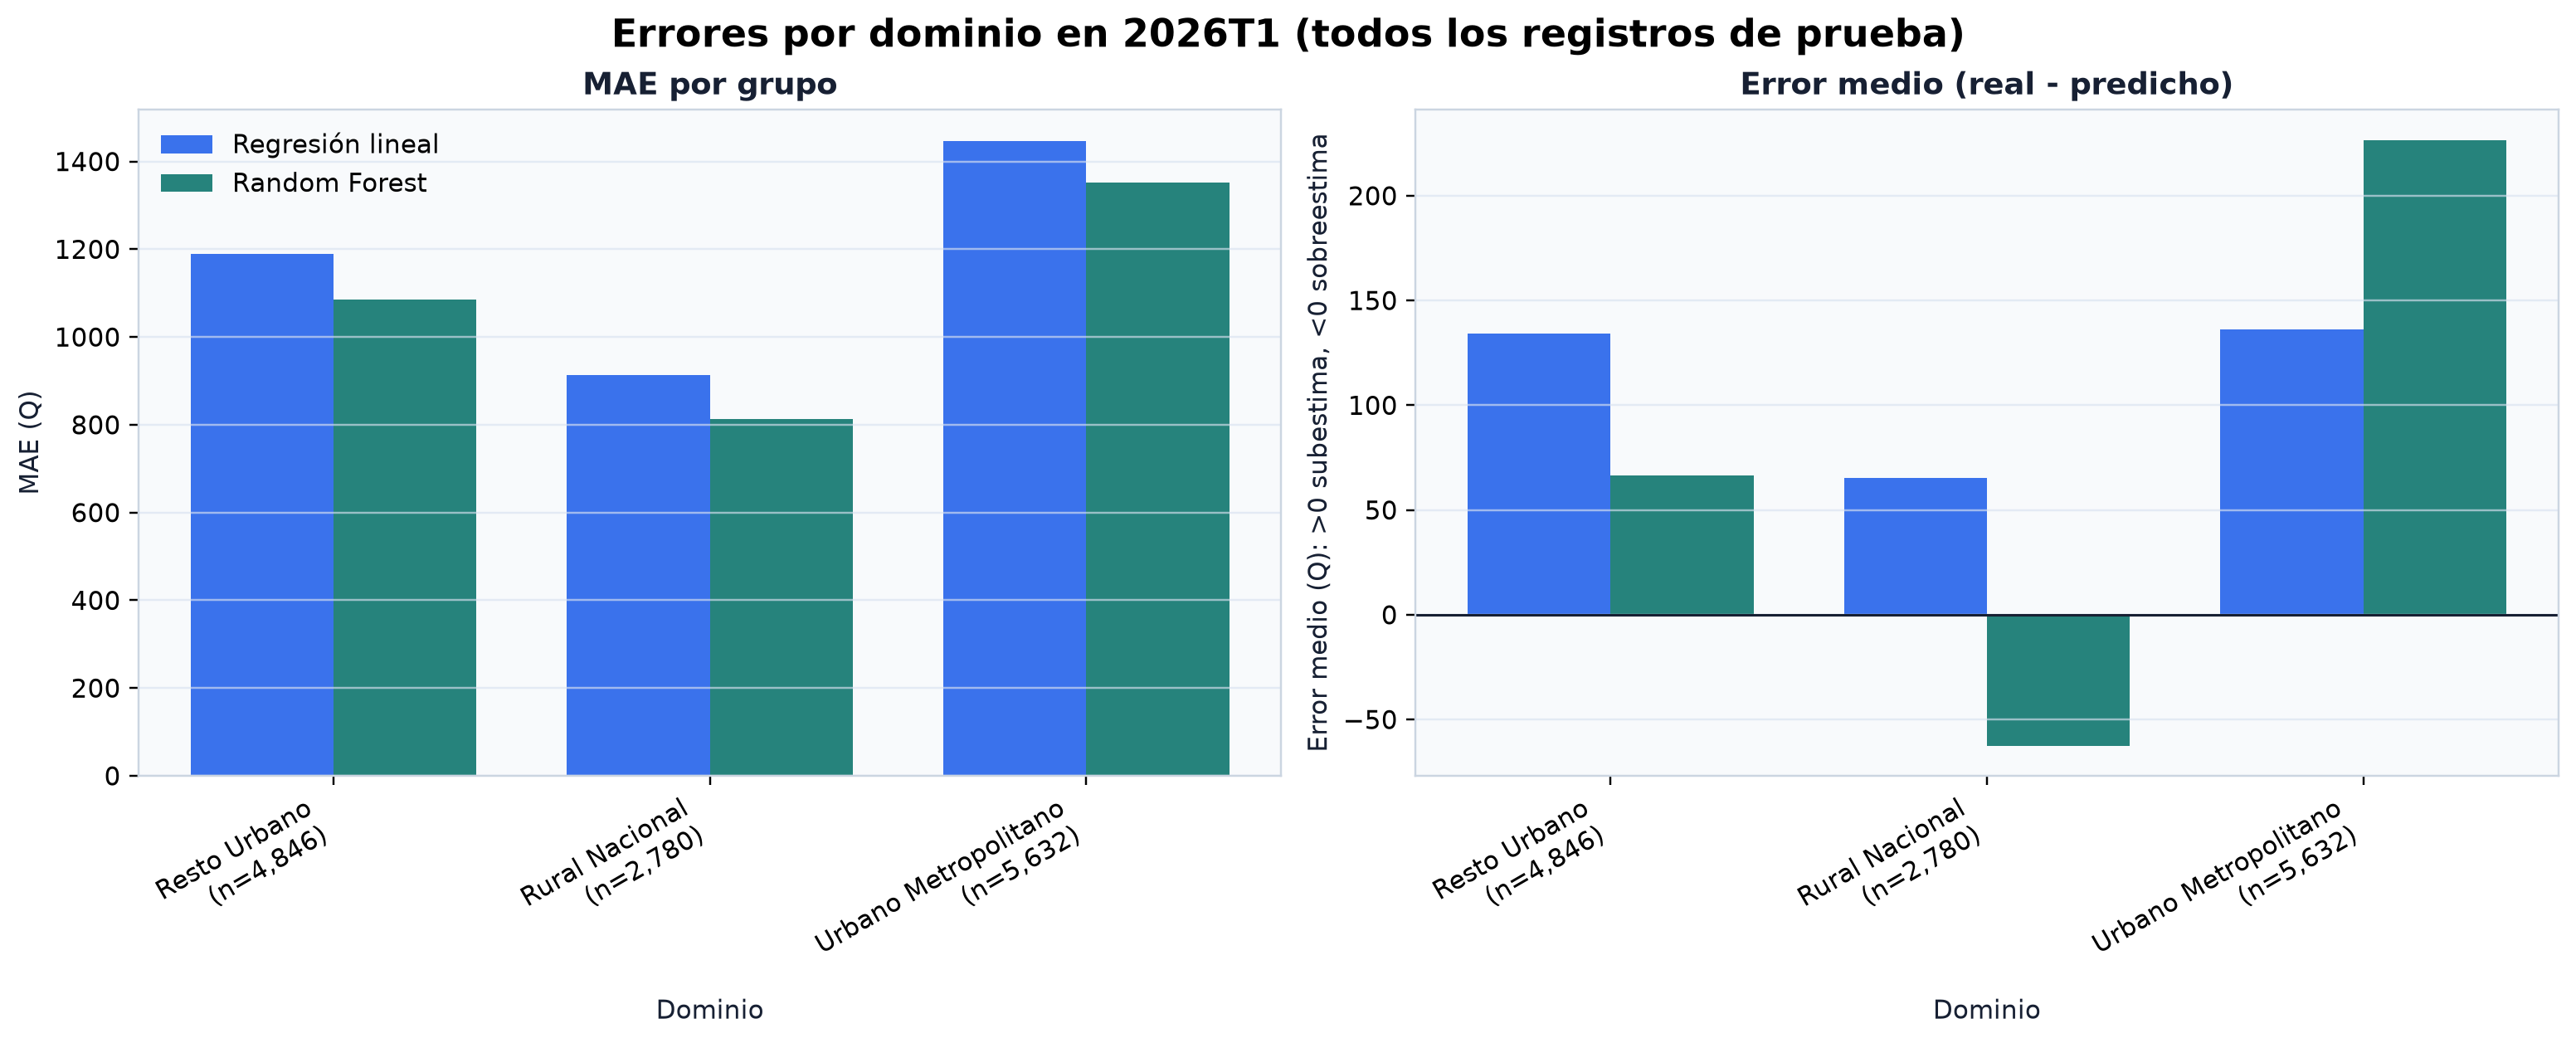
\includegraphics[width=\textwidth]{errores_por_dominio_2026.png}
\caption{MAE y error medio por dominio sobre todo el test.}
\end{figure}

\begin{figure}[htbp]
\centering
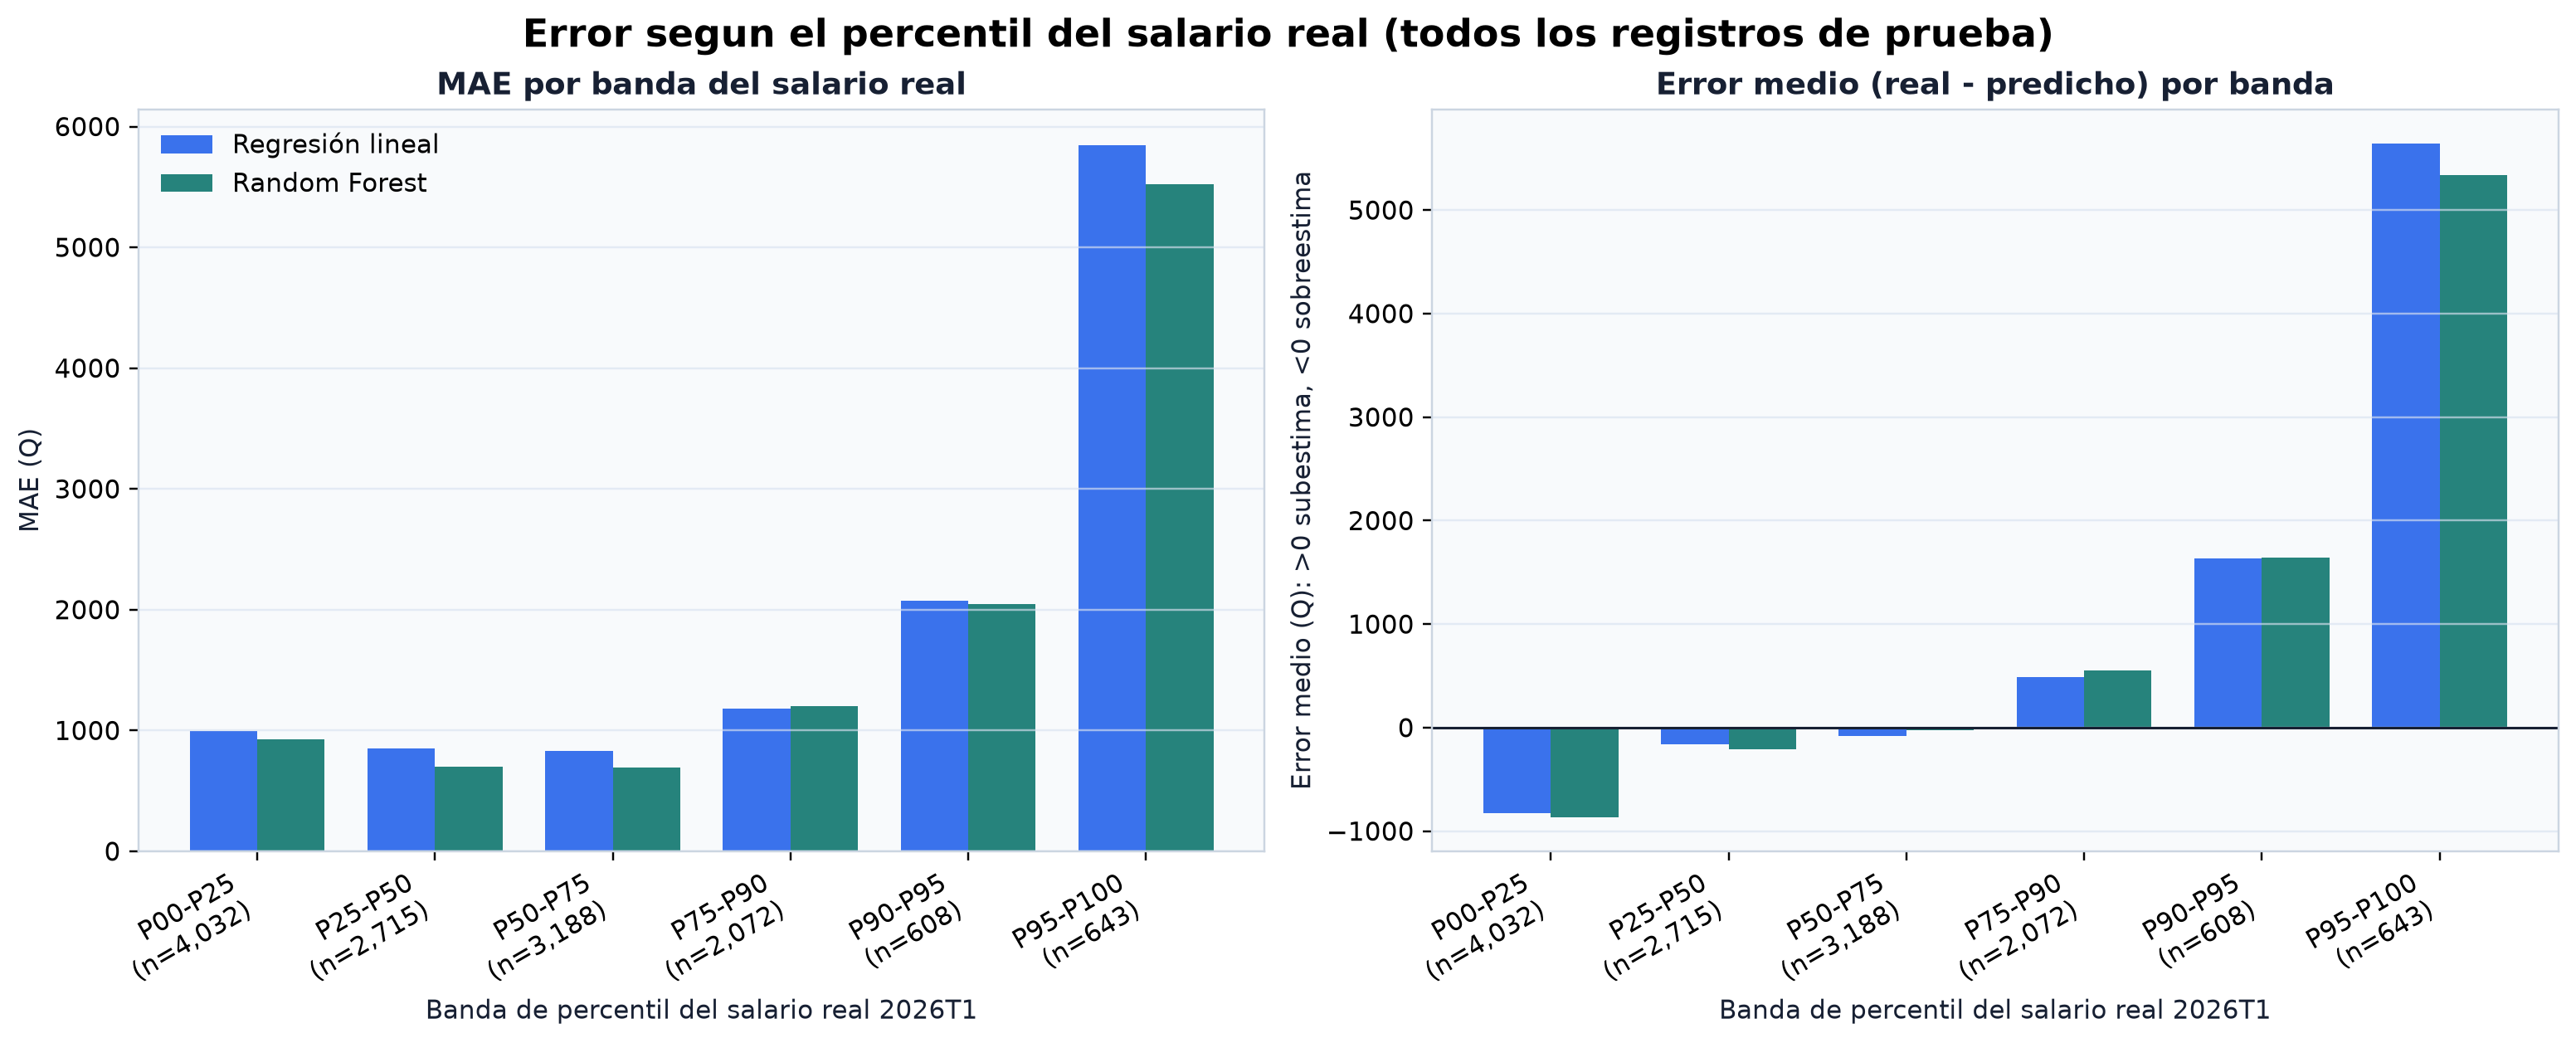
\includegraphics[width=\textwidth]{errores_por_percentil_salarial_2026.png}
\caption{Error según bandas del salario real de 2026T1.}
\end{figure}

\section{Conclusiones y limitaciones}

El analisis identifico perfiles laborales diferenciados y demostro que \textbf{RF\_50\_arboles\_d7} generaliza mejor a 2026T1: MAE Q1,141.51, RMSE Q2,050.55 y $R^2$=0.4887. Su RMSE es 28.59\% menor que el de la referencia y tambien supera a LR\_sin\_regularizacion. La ventaja es compatible con la capacidad del bosque para representar no linealidades e interacciones entre educacion, ocupacion y territorio.

El desempeño no es uniforme. El mayor MAE por educacion se observo en \textbf{Doctorado}, y por dominio en \textbf{Urbano Metropolitano}. En la banda P95-P100, el ganador conserva un MAE de Q5,524.16 y un error medio de Q5,341.04, evidencia de que la cola salarial sigue siendo dificil y tiende a subestimarse. El patron debe interpretarse junto con el tamaño de cada grupo y la regresion a la media.

Las metricas son no ponderadas y describen solamente asalariados elegibles con salario positivo registrado. No representan estimaciones oficiales de Guatemala ni efectos causales. La ausencia de variables como rama de actividad, ocupacion detallada o tamaño de empresa limita la varianza explicada; un uso posterior deberia estudiar estabilidad temporal, equidad por subgrupos y estimaciones ponderadas con FACTOR bajo el diseño muestral correspondiente.


Los resultados son no ponderados y describen solamente los registros
elegibles analizados. No constituyen estimaciones oficiales de la población
guatemalteca ni evidencian relaciones causales. \texttt{FACTOR} se conservó
para documentar el diseño y permitir un análisis poblacional posterior.

\section{Reproducibilidad y fuente}

El notebook se ejecuta de principio a fin, fija semilla 42, mantiene 2026
fuera de la selección y limita pandas a agregados o a la muestra gráfica
permitida. Los Excel, Parquet y modelos se mantienen fuera de Git por tamaño;
el README documenta sus rutas y dependencias.

Instituto Nacional de Estadística de Guatemala. \emph{Encuesta Nacional de
Empleo e Ingresos Continua (ENEIC)}, bases de Personas 2025--2026.\\
\texttt{https://www.ine.gob.gt/encuesta-nacional-de-empleo-e-ingresos/}

\end{document}
